\documentclass[12pt]{article}
\usepackage[table,xcdraw]{xcolor}
\usepackage{multirow}
\usepackage{amsmath}
\usepackage{amsfonts}
\usepackage{float}
\usepackage{fancyhdr}
\usepackage{graphicx}
\usepackage{hyperref}
\usepackage{url}
\usepackage[top=.75in, left=.75in, right=.75in, bottom=1in]{geometry}
\usepackage[utf8]{vietnam}
\usepackage{mathabx}
\usepackage{fontspec}
\usepackage{polyglossia}
\setmainlanguage{vietnamese}
% For algorithm
\usepackage{algorithm}
\usepackage{algpseudocode}

% ============ CODE ============
\usepackage{listings} 
\usepackage{xcolor}
\definecolor{codegreen}{rgb}{0,0.6,0}
\definecolor{codegray}{rgb}{0.5,0.5,0.5}
\definecolor{codepurple}{rgb}{0.58,0,0.82}
\definecolor{backcolour}{rgb}{0.95,0.95,0.92}

% Styling for the code.
\lstdefinestyle{mystyle}{
    backgroundcolor=\color{backcolour},   
    commentstyle=\color{codegreen},
    keywordstyle=\color{magenta},
    numberstyle=\tiny\color{codegray},
    stringstyle=\color{codepurple},
    basicstyle=\ttfamily\footnotesize,
    breakatwhitespace=false,         
    breaklines=true,                 
    captionpos=b,                    
    keepspaces=true,                 
    numbers=left,                    
    numbersep=5pt,                  
    showspaces=false,                
    showstringspaces=false,
    showtabs=false,                  
    tabsize=2
}
\lstset{style=mystyle}
\newcommand{\codefile}[1]{\colorbox{gray!10}{\texttt{#1}}}

% Disable indentation on new paragraphs
\usepackage{indentfirst}
\setlength{\parindent}{2em}
\usepackage[dvipsnames]{xcolor}
% Optional: graphic path
% \graphicspath{PATH_TO_GRAPHIC_FOLDER}

% To use Times font family, uncomment this row
% \usepackage{mathptmx}

% To use roman section / subsection, uncomment these rows
% \renewcommand{\thesection}{\Roman{section}}
% \renewcommand{\thesubsection}{\thesection.\Roman{subsection}}

% Define course name, report name and report title.
\newcommand{\coursename}{An ninh máy tính}
\newcommand{\reportname}{ĐỒ ÁN 1}
\newcommand{\reporttitle}{Báo cáo}

\newcommand{\studentname}{Lê Hoàng Đạt \\ Nguyễn Hồ Đăng Duy \\ Phạm Quang Duy}
\newcommand{\teachername}{Lê Giang Thanh \\ Lê Hà Minh \\ Phan Quốc Kỳ}

% \newcommand{\leftfooter}{\LaTeX\ by Nguyễn Hồ Đăng Duy}
% ============ HEADER AND FOOTER ============
% Header length
\setlength{\headheight}{29.43912pt}

% Footer page number would be on the lower-right corner
\pagestyle{fancy}
\fancyfoot{}
\fancyfoot[R]{Trang \thepage}

\lhead{\reportname}
\rhead{VNUHCMUS\\
\coursename
}


% ============ DOCUMENT ============
\begin{document}
\begin{titlepage}
\newcommand{\HRule}{\rule{\linewidth}{0.5mm}}
\centering

\textsc{\LARGE đại học quốc gia thành phố hồ chí minh}\\[0.8cm]
\textsc{\Large trường đại học khoa học tự nhiên}\\[0.4cm]
\textsc{\large khoa công nghệ thông tin}\\[1cm]

\includegraphics[scale=1.1]{img/hcmus-logo.png}\\[0.8cm] 
\HRule \\[0.4cm]
{ 
\Large{\bfseries{\reporttitle}}\\[0.4cm]
\huge{\bfseries{\reportname}}
}\\[0.4cm]
\HRule \\[0.4cm]

\textbf{\large Môn học: \coursename}\\[0.4cm]
\textbf{\large CSC15003\textunderscore22MMT} \\ [0.7cm]
\begin{minipage}[t]{0.4\textwidth}
\begin{flushleft} \large
\emph{Sinh viên:}\\
\studentname
\end{flushleft}
\end{minipage}
~
\begin{minipage}[t]{0.4\textwidth}
\begin{flushright} \large
\emph{Giảng viên hướng dẫn:} \\
\teachername
\end{flushright}
\end{minipage}\\[0.7cm]

% {\large Tháng 1 năm 2025}\\[1cm]



\vfill
\end{titlepage}
	
\tableofcontents
\pagebreak
\section{Thông tin sinh viên}
Nhóm gồm có 3 thành viên:
\begin{itemize}
    \item 22127060 - Lê Hoàng Đạt - 22127060@student.hcmus.edu.vn

    \item 22127085 - Nguyễn Hồ Đăng Duy - 22127085@student.hcmus.edu.vn

    \item 22127088 - Phạm Quang Duy - 22127088@student.hcmus.edu.vn
\end{itemize}
\section{Giới thiệu}
\textbf{Secure Vault} là một ứng dụng mô phỏng hệ thống bảo mật theo mô hình thực tế, được xây dựng nhằm mục tiêu bảo vệ dữ liệu cá nhân và hỗ trợ truyền tin an toàn giữa người dùng. Ứng dụng tích hợp nhiều kỹ thuật bảo mật hiện đại như mã hóa RSA/AES, xác thực đa yếu tố (MFA), ký số – xác minh chữ ký, QR Code, cùng với cơ chế phân quyền, kiểm tra trạng thái khóa, ghi log bảo mật,...
Người dùng có thể:
\begin{itemize}
    \item Đăng ký, đăng nhập bảo mật với OTP/TOTP
    \item Tạo và quản lý cặp khóa RSA cá nhân
    \item Mã hóa và giải mã tập tin với AES + RSA
    \item Ký số tập tin và xác minh tính toàn vẹn
    \item Tạo và quét QR chứa public key để chia sẻ
    \item Theo dõi trạng thái khóa, phân quyền người dùng (admin/user)
    \item Khôi phục tài khoản khi quên mật khẩu
\end{itemize}

Hệ thống được xây dựng với ngôn ngữ \codefile{Python}, sử dụng \codefile{Flask} cho backend, kết hợp \codefile{MySQL/JSON} để lưu trữ dữ liệu, cùng các thư viện bảo mật như \codefile{pycryptodome, pyotp, qrcode},...

GitHub Repository: https://github.com/YuD1405/Secure\_Vault

\newpage
\section{Phân công chi tiết}
\subsection{Giai đoạn 1: Tìm hiểu và lên kế hoạch}
\renewcommand{\arraystretch}{1.5}
\begin{table}[H]
\centering
\begin{tabular}{|>{\centering\arraybackslash}p{4cm}|>{\arraybackslash}p{9cm}|>{\centering\arraybackslash}p{2.5cm}|}
\hline
\multicolumn{3}{|c|}{\cellcolor[HTML]{FFFFC7}\textbf{Giai đoạn 1: Tìm hiểu và lên kế hoạch}} \\ \hline
\textbf{Thành viên} & 
\multicolumn{1}{>{\centering\arraybackslash}p{9cm}|}{\textbf{Nhiệm vụ}} & 
\textbf{Thời hạn} \\ \hline
Phạm Quang Duy & Tóm tắt thông tin đồ án, chia thành các modules & 16/06 \\ \hline
Phạm Quang Duy  & Tạo repository github và chốt công nghệ & 16/06 \\ \hline
Phạm Quang Duy & Chia task & 16/06 \\ \hline
Cả nhóm & Chốt công nghệ & 16/06 \\ \hline
\end{tabular}
\end{table}

\subsection{Giai đoạn 2: Triển khai chức năng}
\renewcommand{\arraystretch}{1.5}
\begin{table}[H]
\centering
\begin{tabular}{|>{\centering\arraybackslash}p{4cm}|>{\centering\arraybackslash}p{2cm}|>{\arraybackslash}p{7cm}|>{\centering\arraybackslash}p{2.5cm}|}
\hline
\multicolumn{4}{|c|}{\cellcolor[HTML]{DAE8FC}\textbf{QUẢN LÝ NGƯỜI DÙNG}} \\ \hline
\textbf{Thành viên} & \textbf{Yêu cầu} &
\multicolumn{1}{>{\centering\arraybackslash}p{7cm}|}{\textbf{Nhiệm vụ}} & 
\textbf{Thời hạn} \\ \hline
Nguyễn Hồ Đăng Duy &1 & Đăng kí người dùng & 17/06 - 19/06 \\ \hline
Nguyễn Hồ Đăng Duy & 2& Đăng nhập và xác thực MFA & 18/06 - 20/06 \\ \hline
Phạm Quang Duy & 5  & Cập nhật thông tin tài khoản & 20/06 - 21/06 \\ \hline
Nguyễn Hồ Đăng Duy & 10& Phân quyền Admin & 20/06 - 23/06 \\ \hline
Nguyễn Hồ Đăng Duy & 15 &Giới hạn login & 19/06 - 20/06 \\ \hline
Phạm Quang Duy & 17 &Khôi phục tài khoản &  17/06 - 23/06\\ \hline
Nguyễn Hồ Đăng Duy & UI & Frontend: Form accounts, navigation & 29/01 - 09/03 \\ \hline
\end{tabular}
\end{table}

\renewcommand{\arraystretch}{1.5}
\begin{table}[H]
\centering
\begin{tabular}{|>{\centering\arraybackslash}p{4cm}|>{\centering\arraybackslash}p{2cm}|>{\arraybackslash}p{7cm}|>{\centering\arraybackslash}p{2.5cm}|}
\hline
\multicolumn{4}{|c|}{\cellcolor[HTML]{DAE8FC}\textbf{MÃ HÓA VÀ GIẢI MÃ}} \\ \hline
\textbf{Thành viên} & \textbf{Yêu cầu} &
\multicolumn{1}{>{\centering\arraybackslash}p{7cm}|}{\textbf{Nhiệm vụ}} & 
\textbf{Thời hạn} \\ \hline
Lê Hoàng Đạt & 3 & Quản lí khóa & 17/06 - 19/06\\ \hline
Lê Hoàng Đạt & 4 & Tạo và quét QR cho pub key  & 24/06 - 25/06\\ \hline
Lê Hoàng Đạt & 6 & Mã hóa tập tin gửi  &  20/06 - 21/06\\ \hline
Lê Hoàng Đạt & 7 & Giải mã tập tin  & 21/06 - 22/06\\ \hline
Lê Hoàng Đạt & 12 & Chia nhỏ tập tin khi mã hóa &  23/06 - 24/06\\ \hline
Lê Hoàng Đạt & 16 & Tùy chọn định dạng lưu& 21/06 - 22/06 \\ \hline
Phạm Quang Duy & UI & Giao diện chức năng dashboard & 17/06 - 25/06 \\ \hline
\end{tabular}
\end{table}

\renewcommand{\arraystretch}{1.5}
\begin{table}[H]
\centering
\begin{tabular}{|>{\centering\arraybackslash}p{4cm}|>{\centering\arraybackslash}p{2cm}|>{\arraybackslash}p{7cm}|>{\centering\arraybackslash}p{2.5cm}|}
\hline
\multicolumn{4}{|c|}{\cellcolor[HTML]{DAE8FC}\textbf{SIGNING \& LOGGING \& UTILS}} \\ \hline
\textbf{Thành viên} & \textbf{Yêu cầu} &
\multicolumn{1}{>{\centering\arraybackslash}p{7cm}|}{\textbf{Nhiệm vụ}} & 
\textbf{Thời hạn} \\ \hline
Phạm Quang Duy &8 & Ký số & 17/06 - 18/06\\ \hline
Phạm Quang Duy& 9& Xác minh ký số  & 19/06 - 20/06\\ \hline
Phạm Quang Duy & 11  & Log bảo mật  &  21/06 - 22/06\\ \hline
Lê Hoàng Đạt & 13& Kiểm tra trạng thái khóa  & 18/06 - 19/06 \\ \hline
Phạm Quang Duy & 14 &Tìm pub Key & 23/06 - 23/06 \\ \hline
Nguyễn Hồ Đăng Duy & UI &Logging interface & 23/06 - 27/06 \\ \hline
\end{tabular}
\end{table}


% \begin{table}[H]
% \centering
% \begin{tabular}{|>{\centering\arraybackslash}p{4cm}|>{\arraybackslash}p{9cm}|>{\centering\arraybackslash}p{2.5cm}|}
% \hline
% \multicolumn{3}{|c|}{\cellcolor[HTML]{DAE8FC}\textbf{COMPLETE FUNCTIONALITIES}} \\ \hline
% \textbf{Thành viên} &
% \multicolumn{1}{>{\centering\arraybackslash}p{9cm}|}{\textbf{Nhiệm vụ}} & 
% \textbf{Thời hạn} \\ \hline
% Phạm Quang Duy  & Fix Digital signature ( Dò verify với mọi account + Lấy key để kí) & 17/06 - 18/06\\ \hline
% Phạm Quang Duy&FE decrypt để nhận 2 file $\rightarrow$ trả ra thêm biến split / combined & 19/06 - 19/06\\ \hline
% Lê Hoàng Đạt& Chỉnh path encr decr route + module  &  20/06 - 20/06\\ \hline
% Lê Hoàng Đạt & Tách file mã hóa  & 21/06 - 21/06 \\ \hline
% Phạm Quang Duy & Check and manage\_owned\_keys lúc đ + đăng nhập & 22/06 - 22/06 \\ \hline
% Nguyễn Hồ Đăng Duy & UI &Logging interface & 23/06 - 27/06 \\ \hline
% \end{tabular}
% \end{table}

\subsection{Giai đoạn 3: Hoàn thành các chức năng và gộp mã}
\renewcommand{\arraystretch}{1.5}
\begin{table}[H]
\centering
\begin{tabular}{|>{\centering\arraybackslash}p{4cm}|>{\arraybackslash}p{9cm}|>{\centering\arraybackslash}p{2.5cm}|}
\hline
\multicolumn{3}{|c|}{\cellcolor[HTML]{C6EDC3}\textbf{Giai đoạn 3: Hoàn thành các chức năng và merge code}} \\ \hline
\textbf{Thành viên} & 
\multicolumn{1}{>{\centering\arraybackslash}p{9cm}|}{\textbf{Nhiệm vụ}} & 
\textbf{Thời hạn} \\ \hline
Nguyễn Hồ Đăng Duy & Kết nối: Group 1: User management $\rightarrow$ main UI & 01/07 - 03/07\\ \hline
Lê Hoàng Đạt & Kết nối: Group 2: Encrypt và Decrypt $\rightarrow$ main UI & 03/07 - 06/07\\ \hline
Phạm Quang Duy & Kết nối: Group 3: Logging và Utils $\rightarrow$ main UI&  06/07 - 08/07\\ \hline
Phạm Quang Duy & Kết nối toàn bộ chức năng (flow giữa các group chức năng) &  08/07\\ \hline
\end{tabular}
\end{table}

\subsection{Giai đoạn 4: Kiểm thử, viết báo cáo và quay video demo}
\renewcommand{\arraystretch}{1.5}
\begin{table}[H]
\centering
\begin{tabular}{|>{\centering\arraybackslash}p{4cm}|>{\arraybackslash}p{9cm}|>{\centering\arraybackslash}p{2.5cm}|}
\hline
\multicolumn{3}{|c|}{\cellcolor[HTML]{FBA465}\textbf{Giai đoạn 4: Test chức năng, quay video và hoàn thiện report}} \\ \hline
\textbf{Thành viên} & 
\multicolumn{1}{>{\centering\arraybackslash}p{9cm}|}{\textbf{Nhiệm vụ}} & 
\textbf{Thời hạn} \\ \hline
Nguyễn Hồ Đăng Duy & Test toàn bộ flow chương trình &  08/07 - 09/07\\ \hline
Cả nhóm & Chỉnh sửa sau test &   09/07\\ \hline
Cả nhóm & Report &   08/07 - 10/07\\ \hline
Cả nhóm & Record video &  11/07 - 12/07\\ \hline

\end{tabular}
\end{table}

\newpage
\section{Công nghệ sử dụng}

Dưới đây là danh sách các công nghệ và thư viện được sử dụng trong quá trình phát triển ứng dụng \textbf{Secure Vault}, một hệ thống mô phỏng bảo mật gồm xác thực đa yếu tố, mã hóa tập tin, ký số và phân quyền người dùng.

\subsection{Ngôn ngữ lập trình}
\begin{itemize}
    \item \textbf{Python}: Ngôn ngữ chính được sử dụng cho toàn bộ backend của hệ thống.
\end{itemize}

\subsection{Framework}
\begin{itemize}
    \item \textbf{Flask}: Framework web nhẹ, hỗ trợ xây dựng REST API, routing và tích hợp giao diện HTML.
\end{itemize}

\subsection{Thư viện và gói mở rộng}
\begin{itemize}
    \item \texttt{flask}: Framework core cho backend Python.
    \item \texttt{flask-cors}: Cho phép giao tiếp giữa frontend và backend khác nguồn.
    \item \texttt{flask-mysqldb}: Kết nối MySQL với Flask.
    \item \texttt{pyotp}: Tạo và xác minh mã TOTP (Google Authenticator).
    \item \texttt{qrcode}: Tạo mã QR chứa public key hoặc URI xác thực.
    \item \texttt{pillow}: Hỗ trợ xử lý ảnh (dùng kết hợp với QR code).
    \item \texttt{cryptography}: Cung cấp các primitive bảo mật như AES, RSA, SHA-256.
    \item \texttt{python-dotenv}: Quản lý biến môi trường từ file \texttt{.env}.
    \item \texttt{logging} (built-in): Ghi log các hành vi bảo mật, bao gồm đăng nhập, xác thực, mã hóa và các thao tác hệ thống khác    
    \item \texttt{smtplib} (built-in): Giao tiếp với SMTP server để gửi mã OTP qua email.
    \item \texttt{email.mime}: Dùng các class như \texttt{MIMEText}, \texttt{MIMEMultipart} để định dạng nội dung email HTML hoặc plain text.
\end{itemize}

\subsection{Hệ quản trị cơ sở dữ liệu}
\begin{itemize}
    \item \textbf{MySQL}: Lưu trữ thông tin người dùng, khóa, mã OTP và log hành vi bảo mật.
\end{itemize}

\subsection{Công cụ và công nghệ hỗ trợ}
\begin{itemize}
    \item \textbf{Git}: Quản lý phiên bản mã nguồn.
    \item \texttt{.env file}: Lưu cấu hình bảo mật như SMTP, thông tin DB, app secret.
    \item \textbf{SMTP (Gmail App Password)}: Gửi mã OTP qua email.
    \item \textbf{Jinja2}: Template engine giúp render giao diện HTML từ backend Flask.
    \item \textbf{HTML/CSS}: Xây dựng giao diện người dùng cơ bản.
\end{itemize}

\newpage
\section{Kiến trúc hệ thống}
\subsection{Sơ đồ tổng thể}

\subsection{Thư mục và các modules chính}
Đồ án được tổ chức rõ ràng theo mô hình \textbf{Flask MVC} và phân chia modules theo chức năng bảo mật:
\begin{itemize}
    \item \codefile{main.py} - Điểm khởi chạy của ứng dụng \codefile{FLask}
    \item \codefile{.env} - Tập tin cấu hình (thông tin DB, email, secret key,...)
    \item \codefile{data/} - Chứa dữ liệu hệ thống
    \begin{itemize}
        \item \codefile{key\_manage/} - 
        \item \codefile{keys/} - 
        \item \codefile{qr/}
    \end{itemize}
    \item \codefile{flaskapi/} - Backend API
    \begin{itemize}
        \item \codefile{app.py} - Cấu hình Flask app và đăng ký route
        \item \codefile{routes/} - Chứa các tệp định nghĩa route theo nhóm chức năng
    \end{itemize}
    \item \codefile{frontend/} - Các file HTML render giao diện với Jinja2
    \item \codefile{log/} - Ghi toàn bộ hành vi quan trọng: đăng nhập, mã hóa, ký số,... kèm thời gian, email, trạng thái
    \item \codefile{modules/} - Các modules chức năng chính
    \begin{itemize}
        \item \codefile{auth/} - Hash passphrase, sinh OTP, xác thực MFA
        \item \codefile{crypto/} - Mã hóa RSA/AES, ký số và xác minh chữ ký
        \item \codefile{utils/} - Hàm tiện ích chung: log sự kiện, mail, QR,...
    \end{itemize}
    \item \codefile{mySQL/} - Các chương trình để tạo database, table cho cơ sở dữ liệu MySQL
    \item \codefile{report/} - Báo cáo và video demo
    \item \codefile{README.md} - Hướng dẫn cài đặt và chạy thử đồ án. Mô tả các chức năng và công nghệ sử dụng.
\end{itemize}
\newpage
\section{Chi tiết chức năng và kỹ thuật bảo mật}

\subsection{Đăng ký tài khoản người dùng}
\subsubsection*{Mục tiêu}
Cho phép người dùng tạo tài khoản bằng cách điền đầy đủ thông tin cá nhân và \codefile{passphrase} (đảm bảo đủ an toàn). Thông tin sau đó được kiểm tra tính hợp lệ, hash \codefile{passphrase} và lưu vào cơ sở dữ liệu. Đồng thời tạo \codefile{recovery key} và cung cấp cho người dùng.

\subsubsection*{Giao diện}
Giao diện \codefile{/auth/signup} là form HTML bao gồm các trường:
\begin{itemize}
    \item Email
    \item Họ tên
    \item Ngày sinh
    \item Số điện thoại
    \item Địa chỉ
    \item Passphrase và xác nhận passphrase
\end{itemize}
\begin{figure}[H]
\centering
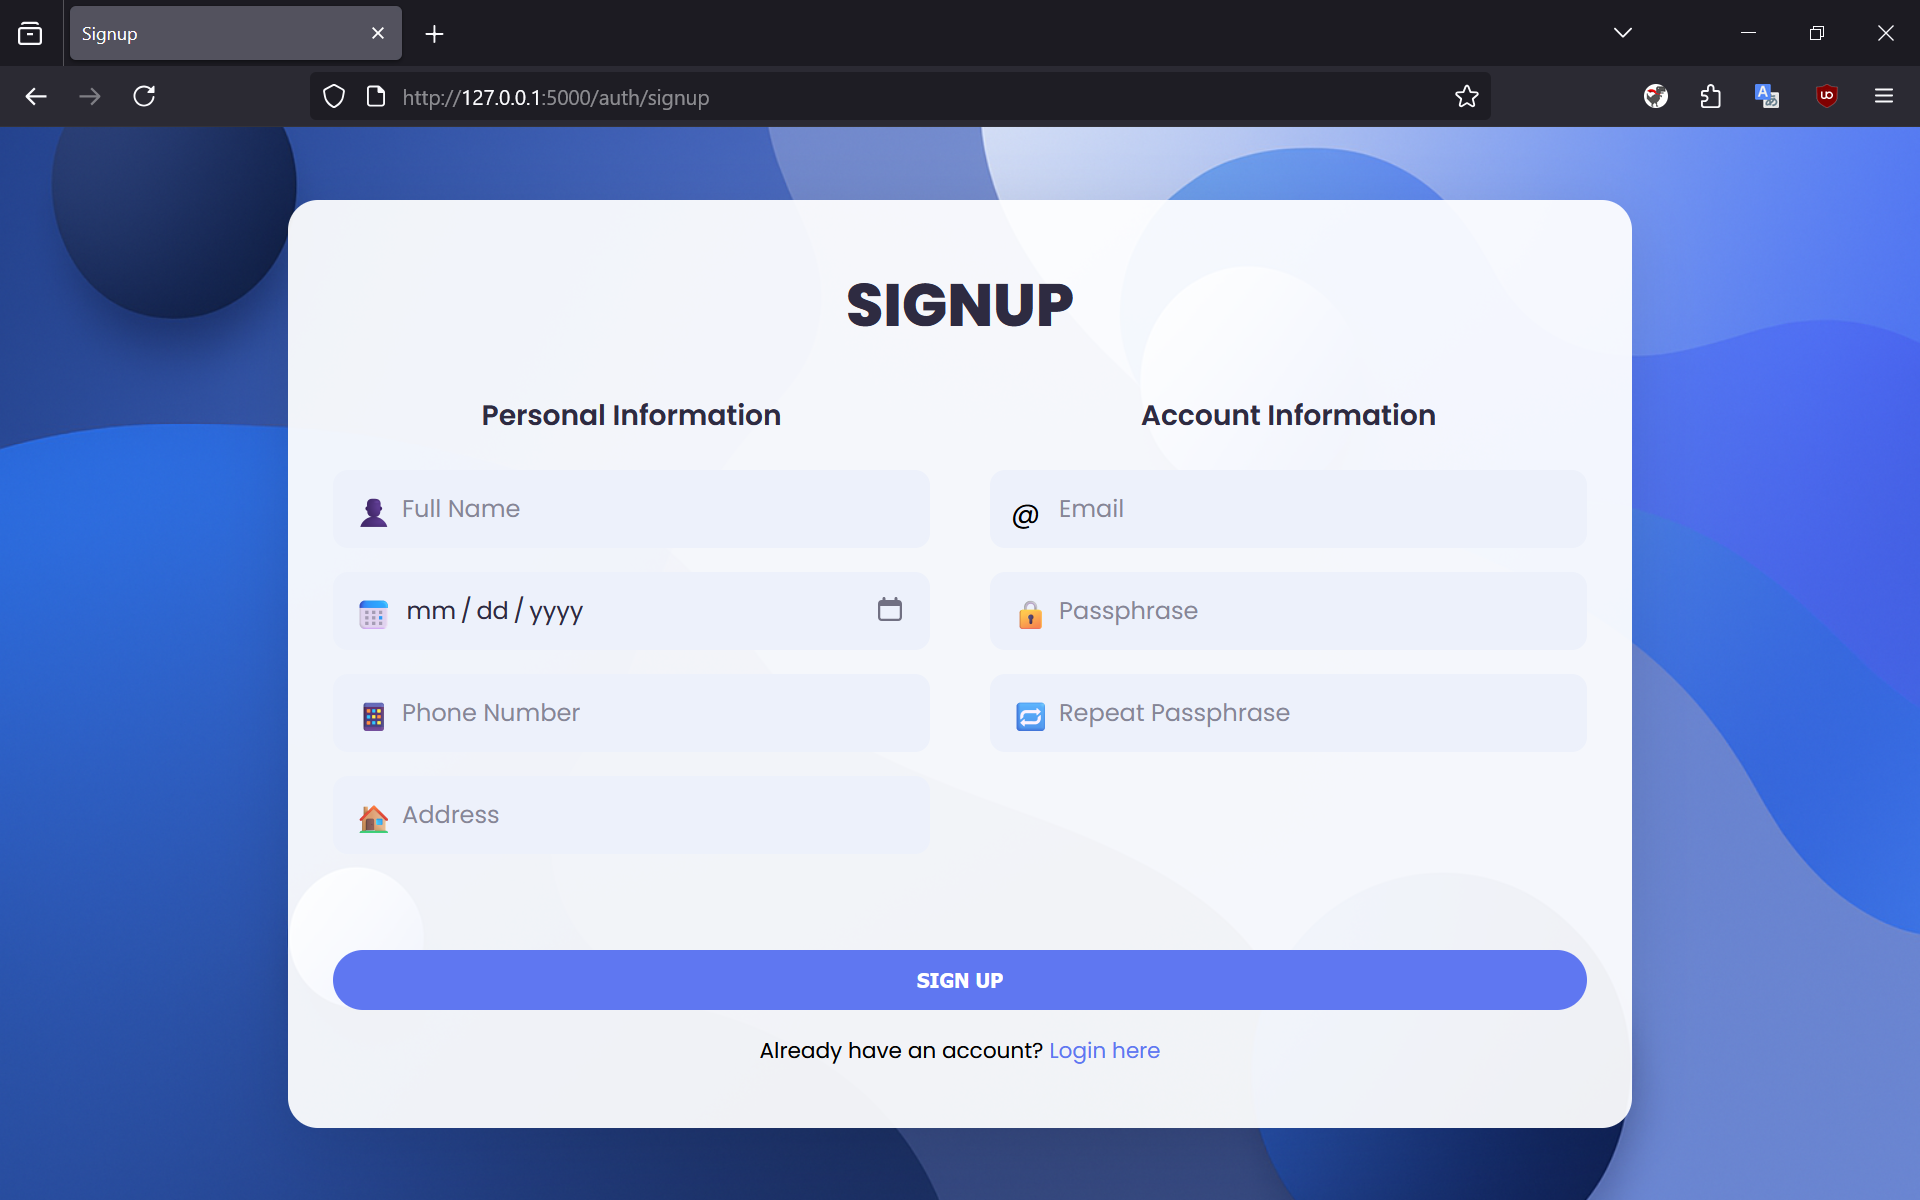
\includegraphics[scale=0.34]{img/sign-up.png}
\caption{Giao diện Signup}
\label{fig:signup_ui}
\end{figure}

Khi đăng ký thành công, hệ thống sẽ hiển thị mã khôi phục tài khoản, yêu cầu người dùng lưu lại mã này để phục hồi nếu mất mật khẩu.
\begin{figure}[H]
\centering
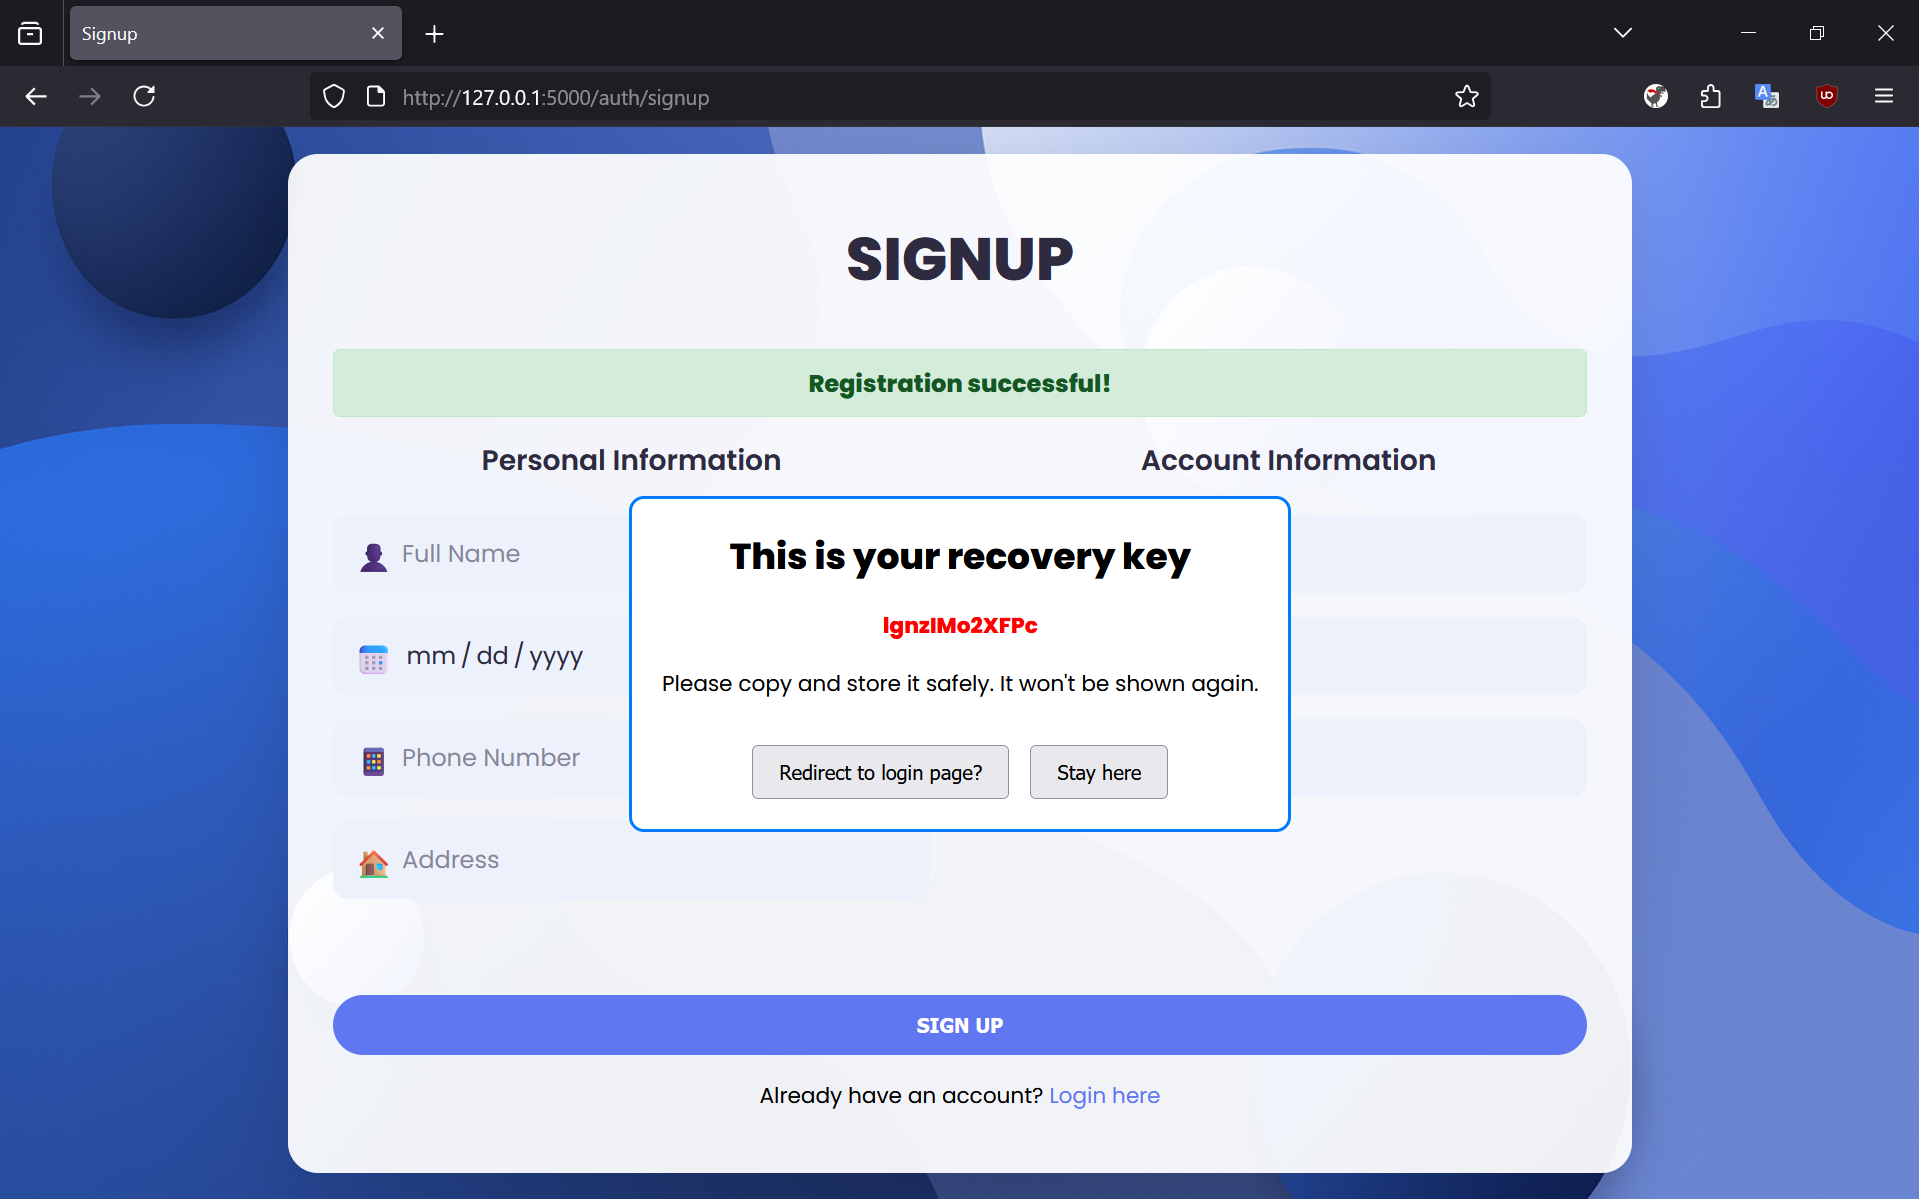
\includegraphics[scale=0.34]{img/recovery-key.png}
\caption{Giao diện popup recovery key}
\label{fig:recovery_key_ui}
\end{figure}

\subsubsection*{Quy trình thực hiện}
\begin{enumerate}
    \item Người dùng nhập thông tin và submit form $\rightarrow$ POST \codefile{/signup}
    \item Flask gọi hàm \codefile{register\_user(request.form)} trong \codefile{logic.py}
    \item Thông tin được kiểm tra và chuẩn hóa:
    \begin{itemize}
        \item Email hợp lệ (\codefile{is\_valid\_email})
        \item Ngày sinh đúng định dạng (\codefile{is\_valid\_date})
        \item Số điện thoại gồm đúng 10 chữ số (\codefile{is\_valid\_phone}) 
        \item Passphrase đủ mạnh (\codefile{is\_strong\_passphrase})
    \end{itemize}
    \item Nếu hợp lệ:
    \begin{itemize}
        \item Sinh \codefile{salt} ngẫu nhiên
        \item Băm \codefile{passphrase} kết hợp với salt bằng \codefile{SHA-256}
        \item Sinh \codefile{recovery\_code} để dùng cho khôi phục
        \item Sinh \codefile{mfa\_secret} phục vụ TOTP trong MFA
    \end{itemize}
    \item Thực hiện \codefile{INSERT} bản ghi vào bảng \codefile{users} trong CSDL
    \item Ghi log hành động: \codefile{log\_user\_action(email, "Register", "Success")}
    \item Trả về kết quả thành công và hiển thị mã khôi phục
\end{enumerate}

\subsubsection*{Chi tiết kỹ thuật và thư viện bảo mật}
\textbf{1. Hashing passphrase với Salt}

Thư viện: \codefile{hashlib, os} 

Kỹ thuật:
\begin{itemize}
    \item Salt được sinh bằng \codefile{os.urandom(16).hex()} $\rightarrow$ đảm bảo tính ngẫu nhiên mạnh.
    \item \codefile{passphrase} được hash bằng \codefile{SHA-256(passphrase + salt)} trước khi lưu xuống DB.
\end{itemize}

\textbf{2.Validator kiểm tra đầu vào}

Thư viện: \codefile{re, datetime} 

Kỹ thuật:
\begin{itemize}
    \item Regex kiểm tra định dạng email, số điện thoại.
    \item Kiểm tra \codefile{passphrase} phải ít nhất 8 ký tự, chứa chữ hoa, số, ký hiệu.
    \item Loại bỏ ký tự nguy hiểm khỏi input (\codefile{sanitize\_input()}) $\rightarrow$ giảm rủi ro XSS / SQLi / Code Injection.
\end{itemize}

\textbf{3. Tạo mã khôi phục}

Thư viện: \codefile{random, string} 

Kỹ thuật:
\begin{itemize}
    \item Sinh chuỗi ngẫu nhiên gồm chữ + số, dùng 1 lần.
    \item Người dùng được yêu cầu lưu lại $\rightarrow$ dùng khi mất \codefile{passphrase}.
    \item Được lưu trong DB (\codefile{users.recovery\_code}) và xóa sau khi reset thành công.
\end{itemize}


\newpage
\subsection{Đăng nhập và Xác thực đa yếu tố (MFA)}
\subsubsection*{Mục tiêu}
Cho phép người dùng đăng nhập bằng cách nhập \codefile{email} và \codefile{passphrase}. Nếu thông tin hợp lệ, hệ thống sẽ yêu cầu xác minh OTP qua email hoặc mã TOTP (Google Authenticator). Hệ thống hỗ trợ các biện pháp bảo mật nâng cao:
\begin{itemize}
    \item Bảo vệ bằng xác thực 2 yếu tố
    \item Tự động khóa tài khoản 5 phút sau 5 lần đăng nhập sai
    \item Cho phép admin khóa tài khoản thủ công
    \item Ghi log toàn bộ hành vi đăng nhập
\end{itemize}
\subsubsection*{Giao diện}
Giao diện \codefile{/auth/login} là form HTML bao gồm 2 trường:
\begin{itemize}
    \item Email
    \item Passphrase
\end{itemize}
\begin{figure}[H]
\centering
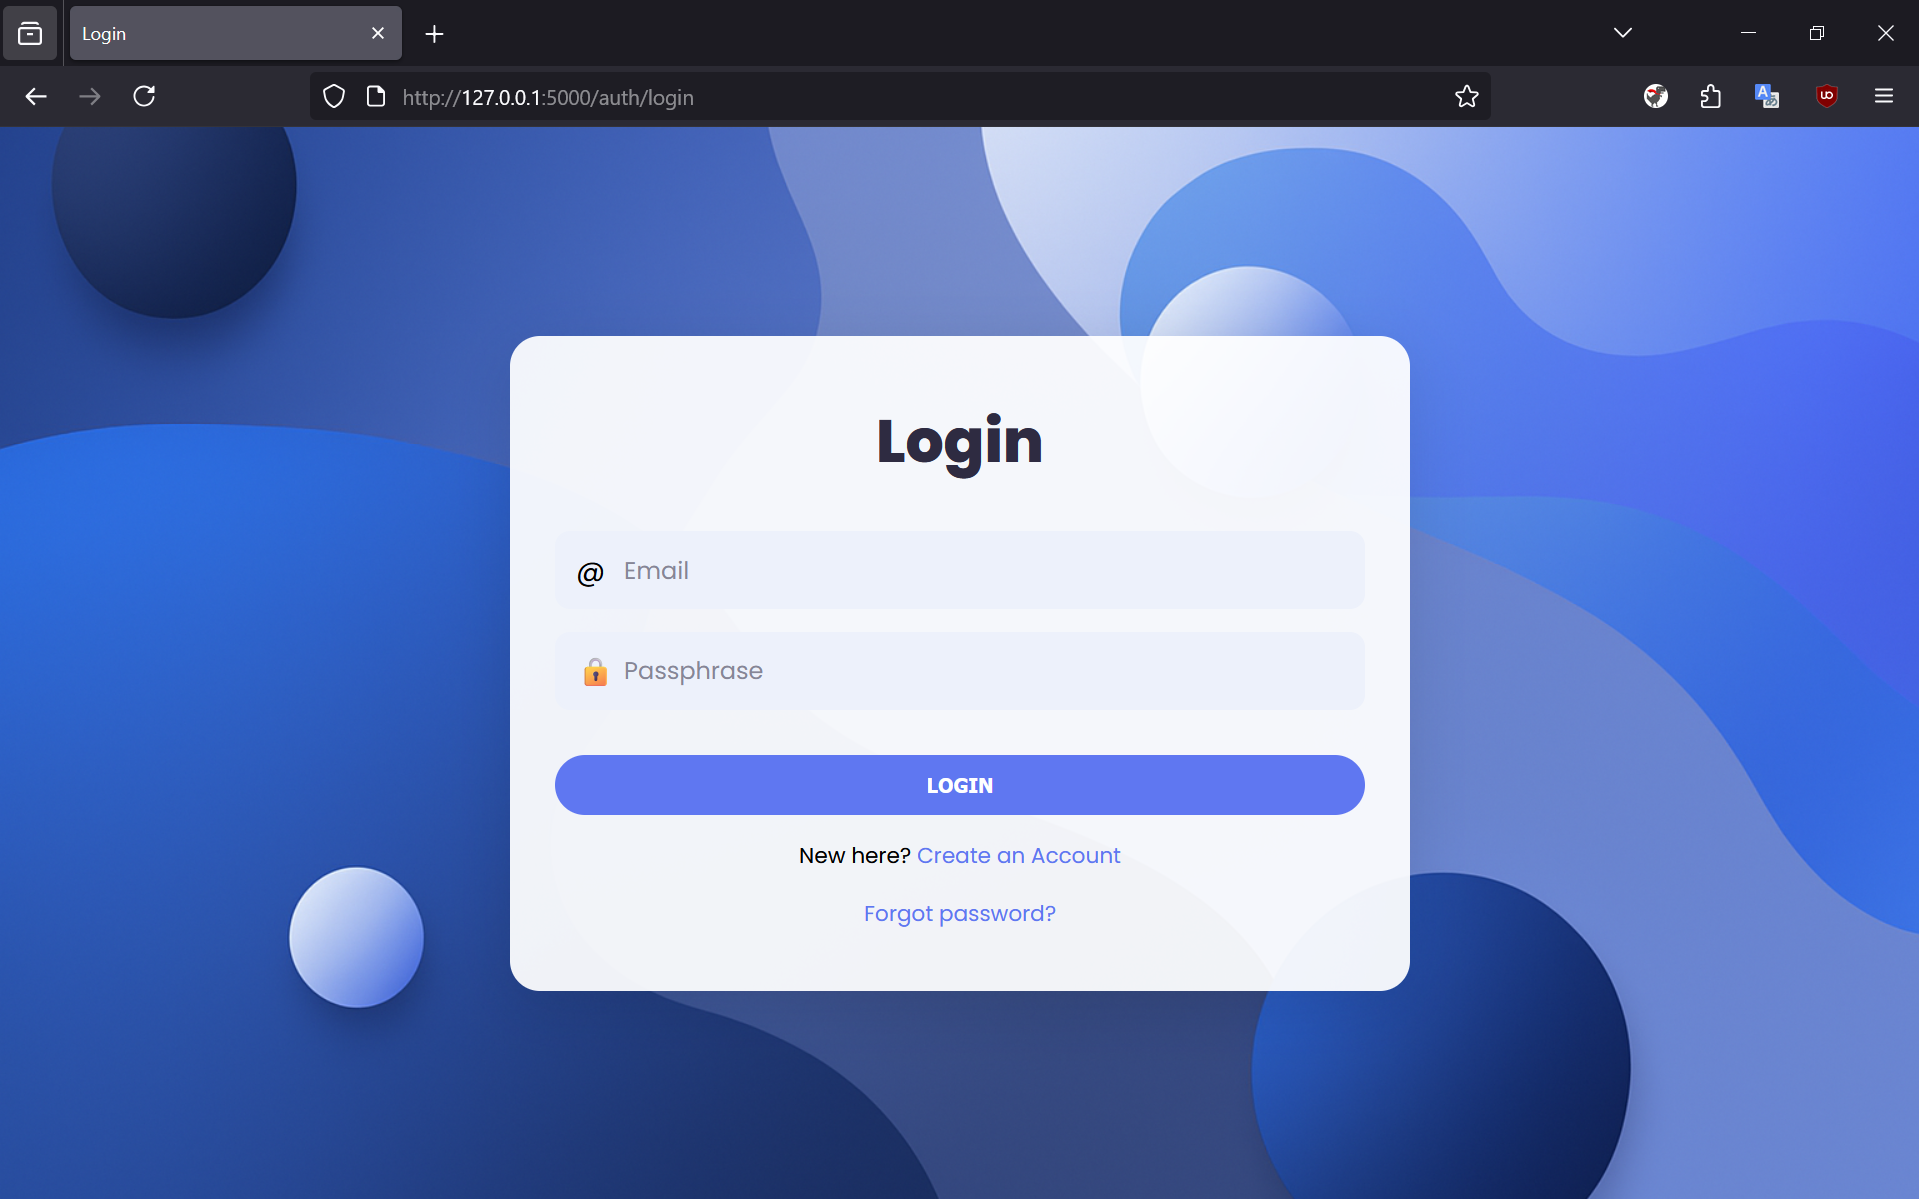
\includegraphics[scale=0.34]{img/login.png}
\caption{Giao diện Login}
\label{fig:login_ui}
\end{figure}

Sau khi đăng nhập thành công, người dùng được chuyển đến \codefile{/auth/verify} để xác thực MFA bằng 1 trong 2 phương thức:
\begin{enumerate}
    \item OTP gửi qua email (mặc định)
    \begin{figure}[H]
    \centering
    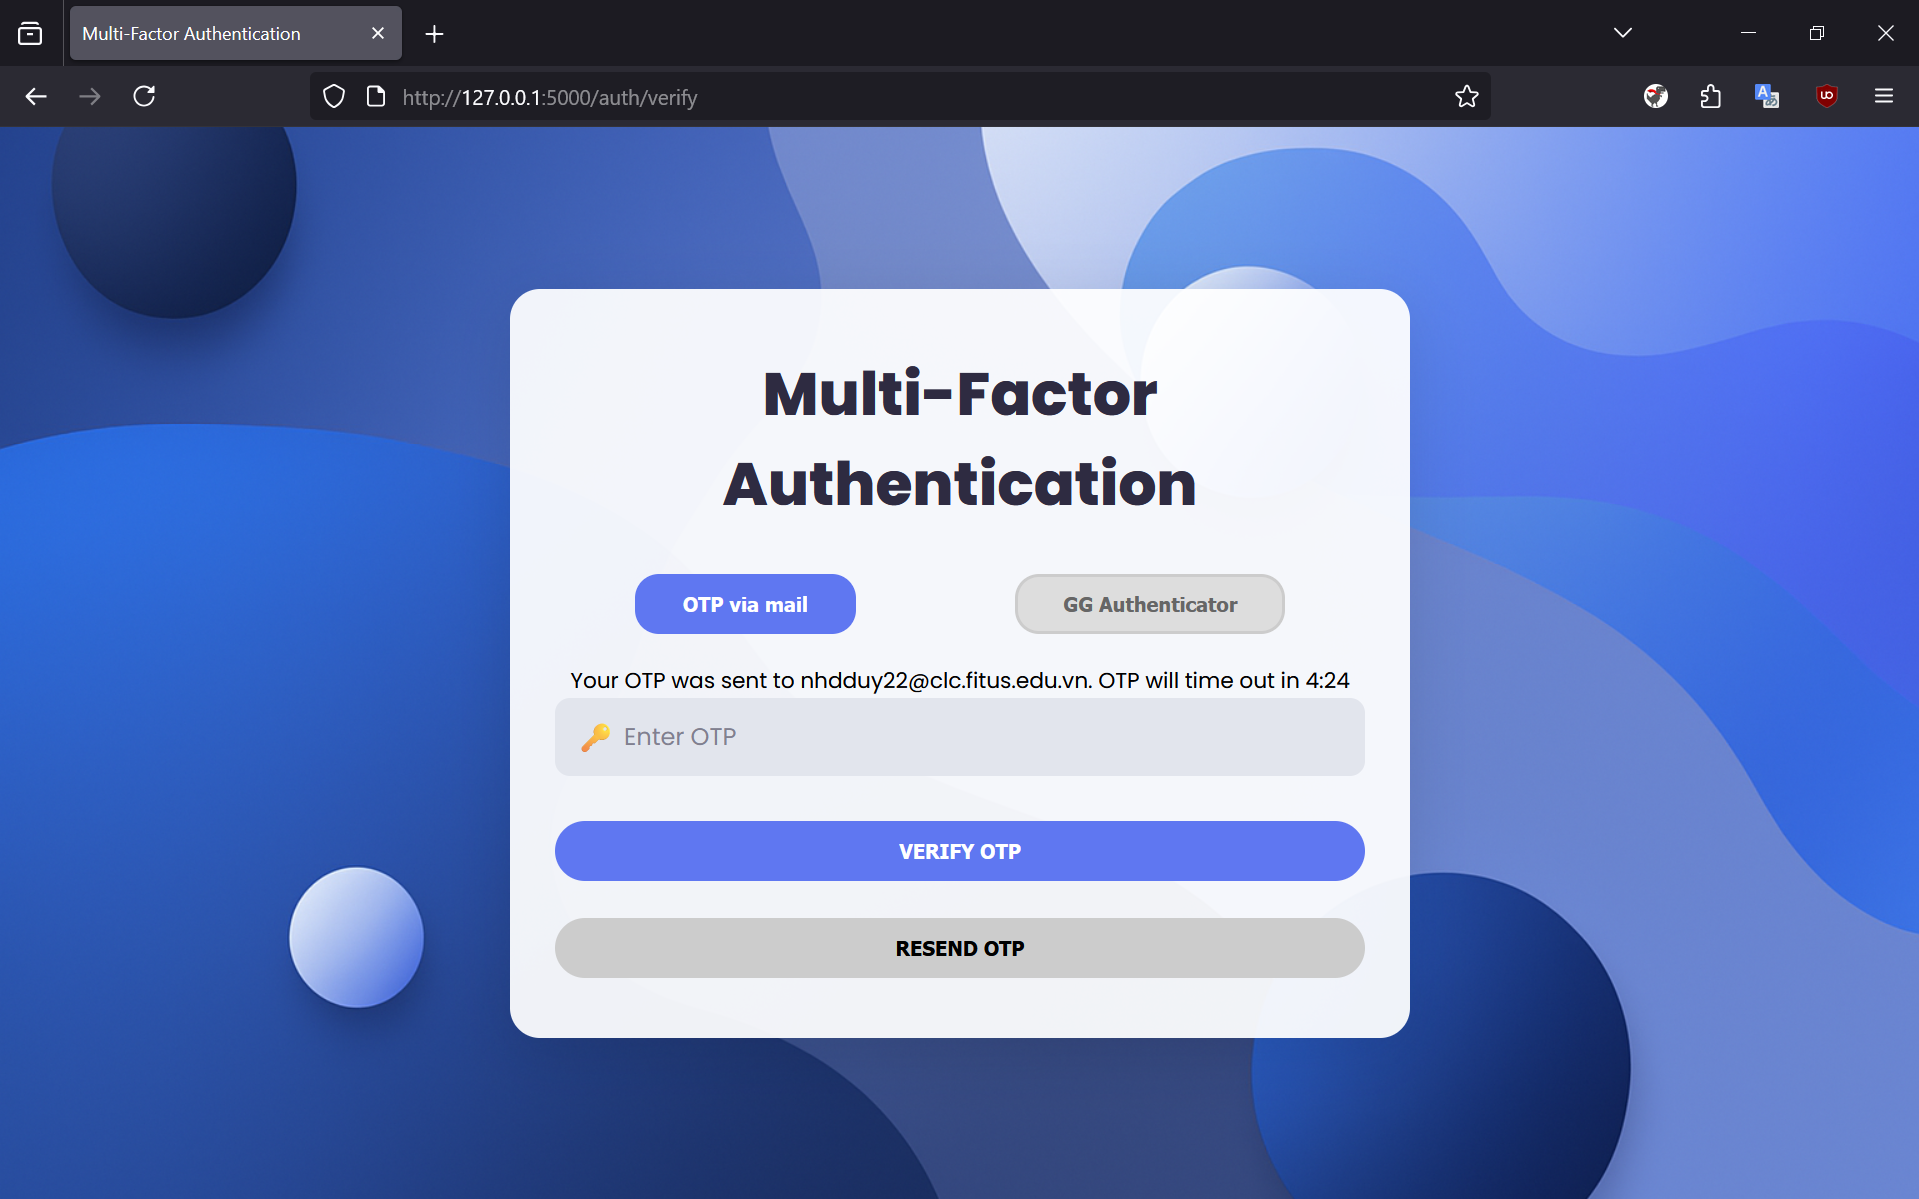
\includegraphics[scale=0.28]{img/MFA-OTP.png}
    \caption{Xác thực bằng OTP gửi qua mail}
    \label{fig:opt_ui}
    \end{figure}
    
    \item Mã TOTP (QR code cho Google Authenticator)
    \begin{figure}[H]
    \centering
    
\includegraphics[scale=0.28]{img/MFA-TOTP.png}
    \caption{Xác thực bằng TOTP qua QR code}
    \label{fig:totp_ui}
    \end{figure}
\end{enumerate}

\subsubsection*{Quy trình thực hiện}
\begin{enumerate}
    \item Người dùng submit form \codefile{/auth/login} với \codefile{email} và \codefile{passphrase}.
    \item Flask gọi hàm \codefile{process\_login(email, passphrase) )} trong \codefile{logic.py}
    \item Chương trình thực hiện:
    \begin{itemize}
        \item Kiểm tra người dùng tồn tại hay không.
        \item So sánh \codefile{hash(passphrase + salt)}.
        \item Nếu sai, tăng \codefile{failed\_attempts} và cập nhật \codefile{last\_failed\_login}. 
        \item Nếu sai hơn 5 lần trong 2 phút $\rightarrow$ Gán \codefile{is\_locked = 1}, trả về trạng thái \textbf{locked}.
        \item Nếu tài khoản bị khóa bởi admin (\codefile{last\_failed\_login = null} và \codefile{is\_locked = 1}) $\rightarrow$ trả về \textbf{locked by admin}.
        \item Nếu các thông tin đăng nhập đúng $\rightarrow$ Reset \codefile{failed\_attempts}, ghi log, chuyển đến bước xác thực MFA.
    \end{itemize}
    \item Người dùng được chuyển đến \codefile{/auth/verify}, chọn xác thực OTP qua email hoặc quét QR TOTP (mặc định là gửi OTP qua email đã đăng ký).
    \item Nếu chọn OTP:
    \begin{itemize}
        \item Gọi \codefile{generate\_and\_send\_otp(email)} $\rightarrow$ sinh mã 6 chữ số, gửi qua email, lưu DB kèm thời gian hết hạn.
        \begin{figure}[H]
        \centering
        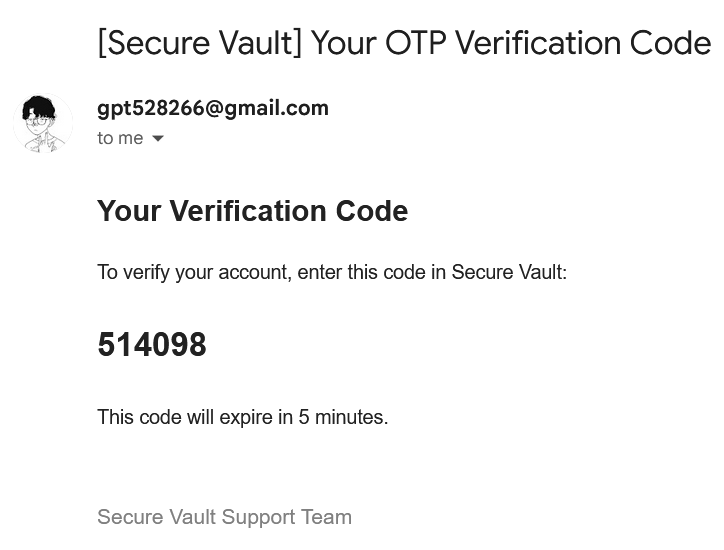
\includegraphics[scale=0.34]{img/mail-otp.png}
        \caption{Cấu trúc mail}
        \label{fig:mail_recovery_ui}
        \end{figure}
        \item Kiểm tra bằng \codefile{verify\_otp\_code(email, input\_code)}.
    \end{itemize}
    \item Nếu chọn TOTP:
    \begin{itemize}
        \item Sinh mã QR từ \codefile{generate\_qr\_code(email)} $\rightarrow$ dùng cho ứng dụng Google Authenticator.
        \item Kiểm tra bằng \codefile{verify\_totp\_code(email, input\_code)}.
    \end{itemize}
    \item Nếu đúng $\rightarrow$ Lưu \codefile{session['user\_id]} và chuyển đến \codefile{auth/dashboard}
\end{enumerate}

\subsubsection*{Chi tiết kỹ thuật và thư viện bảo mật}
\textbf{1. Hashing passphrase với Salt}

Thư viện: \codefile{hashlib} 

Kỹ thuật:
\begin{itemize}
    \item Salt đã được sinh bằng \codefile{os.urandom(16).hex()} $\rightarrow$.
    \item Kiểm tra \codefile{passphrase} được người dùng nhập vào sau khi hash có giống với chuỗi được lưu trong DB hay không.
\end{itemize}

\textbf{2. Gửi mã OTP qua email}

Thư viện: \codefile{random, datetime, smtplib, email} 

Kỹ thuật:
\begin{itemize}
    \item Sinh mã 6 chữ số ngẫu nhiên.
    \item Lưu \codefile{expires\_at = now + 5 minutes}
    \item Dùng \codefile{email.mime.text} và \codefile{email.mime.multipart} để format tin nhắn gửi email.
    \item Tạo tài khoản gmail đã xác thực 2 yếu tố và tiến hành tạo \codefile{app password} và lưu vào \codefile{.env} với cấu trúc như sau
\begin{lstlisting}
SMTP_USER=<sender mail>
SMTP_PASS=<app password>
\end{lstlisting}
    \item OTP được tạo sẽ lưu vào DB và gửi bằng SMTP $\rightarrow$ người dùng cần kiểm tra email để nhận OTP.
    \item Người dùng nhập mã OTP $\rightarrow$ Server sẽ lấy bản \codefile{otp\_code} mới nhất và kiểm tra xem mã có đúng và còn hạn hay không $\rightarrow$ Nếu hợp lệ, người dùng xác thực thành công
\end{itemize}

\textbf{3. TOTP}

Thư viện: \codefile{pyotp, qrcode, base64} 

Kỹ thuật:
\begin{itemize}
    \item Mỗi tài khoản có một \codefile{mfa\_secret} (chuỗi \codefile{base32}) sinh ngẫu nhiên và được lưu trong bảng \codefile{users}.
    \item Dùng \codefile{pyotp.totp.TOTP(mfa\_secret).provisioning\_uri()} để tạo ra URI định dạng chuẩn TOTP.
    \item Sinh ảnh QR code từ URI trên.
    \item Người dùng sử dụng Google Authenticator để quét mã trên.
    \item Người dùng nhập 6 số do app tạo ra mỗi 30 giây.
    \item Server sẽ dùng lại \codefile{mfa\_secret} từ DB để sinh lại mã đúng tại thời điểm đó. Nếu mã số giống nhau thì người dùng xác thực thành công.
\end{itemize}
\newpage

\subsection{Quản lý khoá RSA cá nhân}
\subsubsection*{Mục tiêu}

\subsubsection*{Giao diện}

\subsubsection*{Quy trình thực hiện}

\subsubsection*{Chi tiết kỹ thuật và thư viện bảo mật}
\newpage

\subsection{QR Code Public Key}
\subsubsection*{Mục tiêu}

\subsubsection*{Giao diện}

\subsubsection*{Quy trình thực hiện}

\subsubsection*{Chi tiết kỹ thuật và thư viện bảo mật}
\newpage
\subsection{Cập nhật thông tin tài khoản}

\subsubsection*{Mục tiêu}
Chức năng cập nhật tài khoản cho phép người dùng chỉnh sửa thông tin cá nhân (họ tên, ngày sinh, địa chỉ, số điện thoại), cũng như thay đổi mật khẩu (passphrase). Việc này đảm bảo:
\begin{itemize}
    \item Người dùng có thể chủ động thay đổi thông tin cá nhân khi cần.
    \item Cho phép cập nhật passphrase và tự động mã hóa lại khóa RSA bằng passphrase mới.
    \item Đảm bảo tính bảo mật và tính nhất quán dữ liệu khóa trong hệ thống.
\end{itemize}

\subsubsection*{Giao diện}
Giao diện tại \texttt{/render\_update\_account} bao gồm:
\begin{itemize}
    \item Form nhập các trường: Họ tên, ngày sinh, địa chỉ, số điện thoại.
    \item Tùy chọn nhập mật khẩu hiện tại và mật khẩu mới nếu muốn đổi passphrase.
    \item Nút \texttt{Save changes} sẽ gửi POST đến API \texttt{/update\_account} và hiển thị thông báo kết quả.
\end{itemize}

\begin{figure}[H]
    \centering
    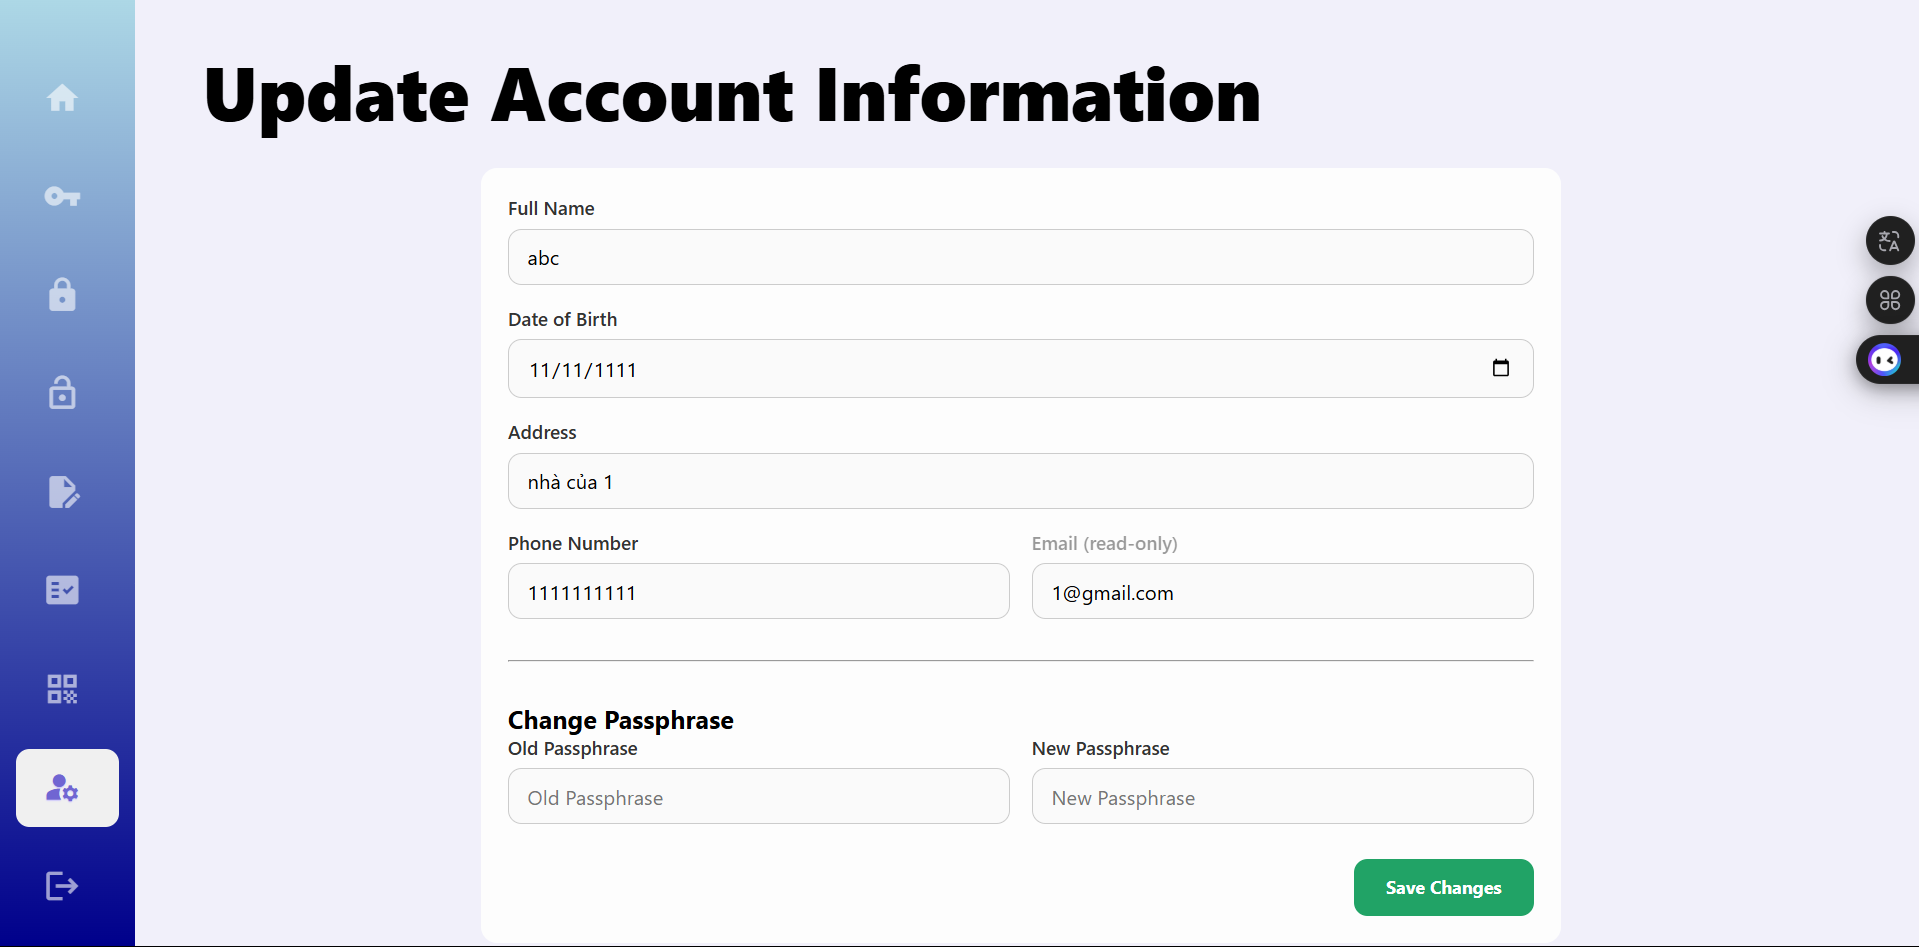
\includegraphics[width=0.85\textwidth]{img/5_update/5_update_form.png}
    \caption{Giao diện cập nhật thông tin}
\end{figure}

\subsubsection*{Quy trình thực hiện}
\begin{description}

    \item[\textbf{Bước 1 - Người dùng nhập thông tin}]
    Người dùng điền thông tin cần thay đổi, có thể chọn thay đổi passphrase hoặc không.

    \item[\textbf{Bước 2 - Gửi yêu cầu cập nhật}]
    Form gửi POST đến route \texttt{/update\_account}, kèm theo session để xác định người dùng.

    \item[\textbf{Bước 3 - Kiểm tra và xử lý}]
    Server thực hiện:
    \begin{itemize}
        \item Kiểm tra dữ liệu đầu vào và định dạng.
        \item Kiểm tra passphrase cũ nếu có yêu cầu đổi mật khẩu.
        \item Hash passphrase mới và cập nhật.
        \item Nếu đổi mật khẩu, khóa riêng RSA sẽ được giải mã bằng passphrase cũ và mã hóa lại bằng passphrase mới.
    \end{itemize}

    \item[\textbf{Bước 4 - Ghi log và phản hồi}]
    Ghi log cập nhật tài khoản và trả kết quả thành công hoặc thất bại cho giao diện frontend.

    \begin{figure}[H]
        \centering
        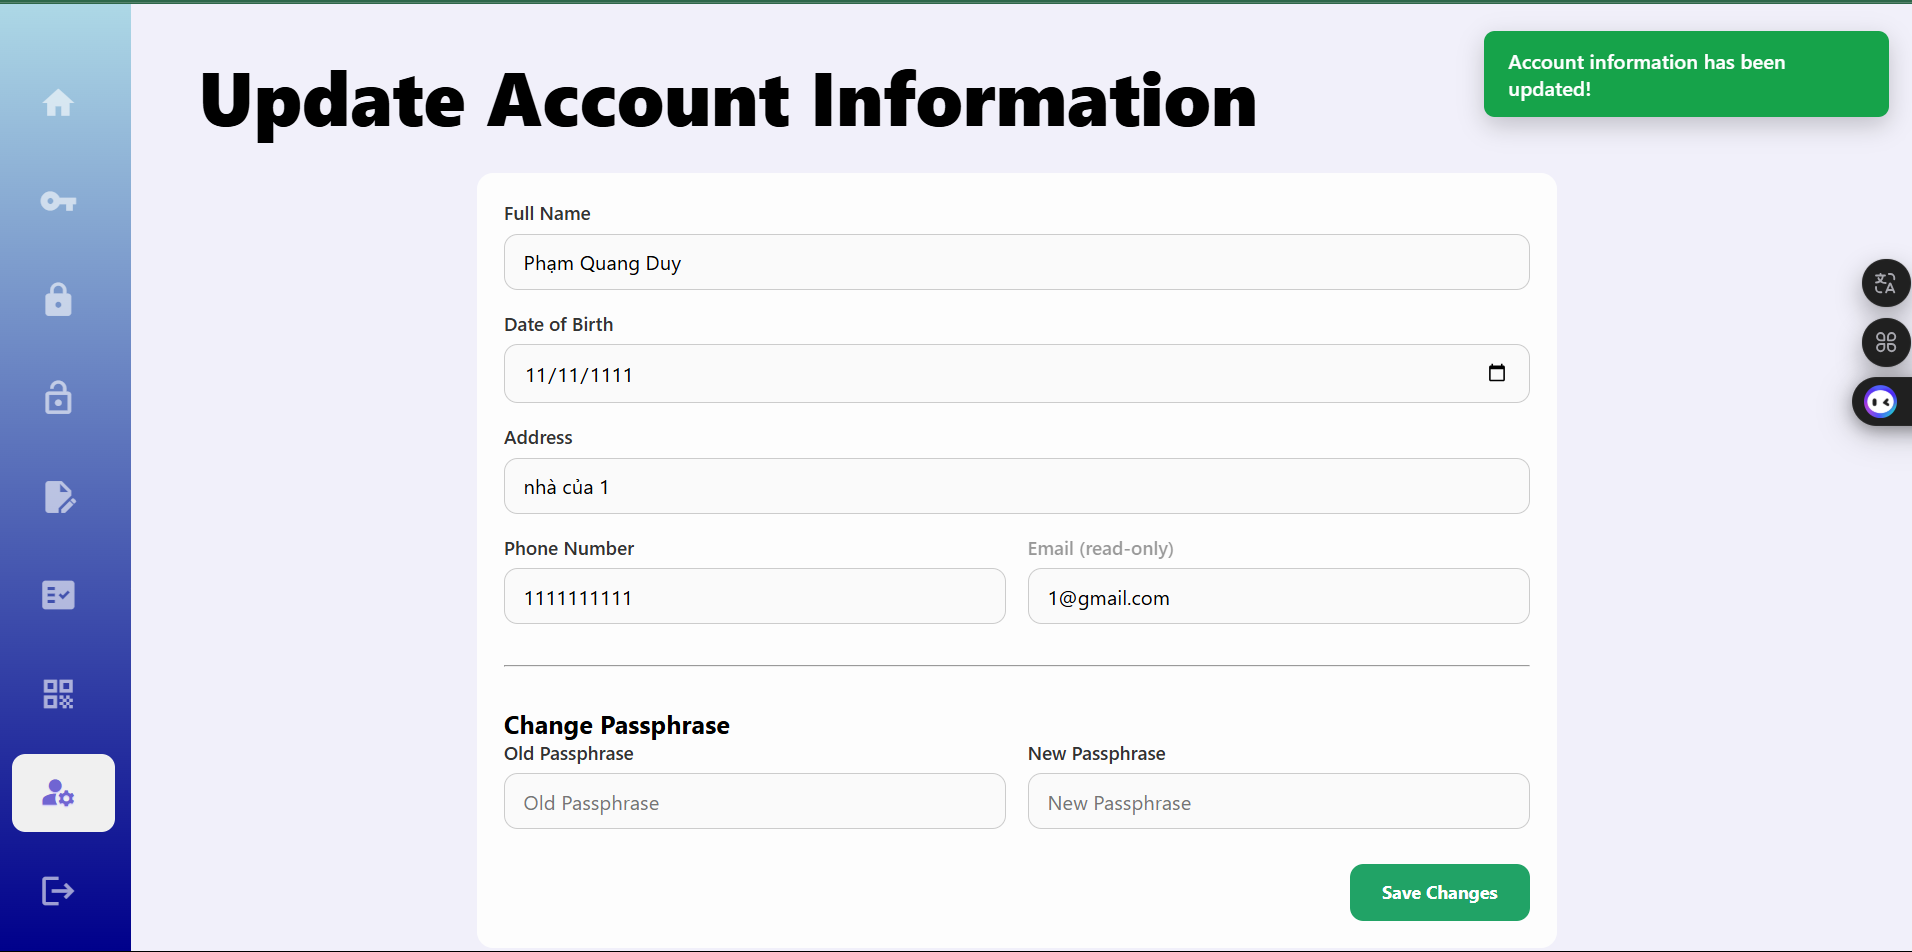
\includegraphics[width=0.85\textwidth]{img/5_update/5_update_success.png}
        \caption{Giao diện cập nhật thông tin thành công}
    \end{figure}
\end{description}

\subsubsection*{Chi tiết kỹ thuật và thư viện bảo mật}
\begin{description}

    \item[\textbf{1. Kiểm tra thông tin đầu vào}]
    \begin{itemize}
        \item Sử dụng các hàm xác thực định dạng: \texttt{is\_valid\_email()}, \texttt{is\_valid\_date()}, \texttt{is\_valid\_phone()}.
        \item Bắt buộc điền đầy đủ thông tin: email, họ tên, ngày sinh, địa chỉ, số điện thoại.
    \end{itemize}

    \item[\textbf{2. Kiểm tra và cập nhật passphrase}]
    \begin{itemize}
        \item Nếu có ý định đổi passphrase, yêu cầu nhập cả pass cũ và pass mới.
        \item Pass mới phải khác pass cũ và đạt yêu cầu bảo mật qua hàm \texttt{is\_strong\_passphrase()}.
        \item So sánh hash passphrase cũ với DB bằng \texttt{hash\_with\_salt()}.
        \item Nếu hợp lệ, hash passphrase mới và cập nhật vào DB.
    \end{itemize}

    \item[\textbf{3. Re-encrypt RSA key với passphrase mới}]
    \begin{itemize}
        \item Hàm \texttt{re\_encrypt\_private\_key\_with\_new\_passphrase()} dùng để giải mã khóa RSA bằng passphrase cũ và mã hóa lại bằng passphrase mới.
        \item Nếu lỗi trong quá trình này, cập nhật DB sẽ được rollback và trả lỗi.
        \item Passphrase mới được cập nhật vào session để sử dụng cho các thao tác sau.
    \end{itemize}
    \begin{figure}[H]
        \centering
        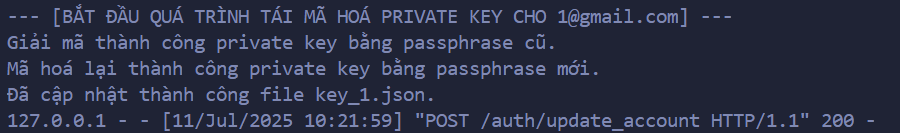
\includegraphics[width=0.85\textwidth]{img/5_update/5_update_re_enc.png}
        \caption{Mã hóa passphrase mới thành công}
    \end{figure}

    \item[\textbf{4. Cập nhật recovery key (khóa khôi phục)}]
    Để đảm bảo người dùng có thể khôi phục khóa riêng sau khi quên passphrase, hệ thống sử dụng một \textbf{recovery key} (AES key phụ) được mã hóa bằng passphrase hiện tại. Khi người dùng thay đổi passphrase, recovery key cần được giải mã và mã hóa lại như sau:

    \begin{itemize}
        \item \textbf{Bước 1: Giải mã recovery key bằng passphrase cũ}
        \begin{itemize}
            \item Truy vấn trường \texttt{encrypted\_recovery\_key} từ bảng \texttt{users}.
            \item Derive khóa AES từ passphrase cũ bằng hàm \texttt{derive\_aes\_key(pass1, salt)}.
            \item Giải mã recovery key hiện tại bằng AES.
        \end{itemize}

        \item \textbf{Bước 2: Mã hóa lại recovery key bằng passphrase mới}
        \begin{itemize}
            \item Derive AES key mới từ passphrase mới: \texttt{derive\_aes\_key(pass2, salt)}.
            \item Mã hóa recovery key vừa giải mã bằng AES key mới.
            \item Lưu bản mã hóa mới vào trường \texttt{encrypted\_recovery\_key}.
        \end{itemize}

        \item \textbf{Lưu ý bảo mật:}
        \begin{itemize}
            \item Nếu giải mã hoặc mã hóa recovery key thất bại, toàn bộ quá trình cập nhật sẽ bị rollback và trả lỗi.
            \item Mọi thao tác đều được log bằng \texttt{log\_user\_action(..., "Fail", ...)} hoặc \texttt{log\_internal\_event()} với mức \texttt{error}.
        \end{itemize}
    \end{itemize}

    \item[\textbf{5. Ghi log và bảo mật}]
    \begin{itemize}
        \item Mọi thao tác đều được ghi bằng \texttt{log\_user\_action()} với trạng thái và chi tiết lỗi.
        \item Lỗi truy cập không có session sẽ chuyển hướng về trang đăng nhập.
        \item Dữ liệu passphrase luôn được hash bằng salt, không lưu dưới dạng thô.
    \end{itemize}

    \item[\textbf{6. Xử lý lỗi}]
    \begin{itemize}
        \item Nếu thiếu session → lỗi 401 hoặc redirect về trang đăng nhập.
        \item Nếu định dạng sai hoặc passphrase cũ không đúng → trả lỗi rõ ràng.
        \item Nếu không có thay đổi gì → trả thông báo: \texttt{"No changes were made."}
        \item Nếu cập nhật thành công nhưng RSA re-encryption thất bại → rollback và log lỗi mức độ \texttt{error}.
    \end{itemize}

    
    \begin{figure}[H]
        \centering
        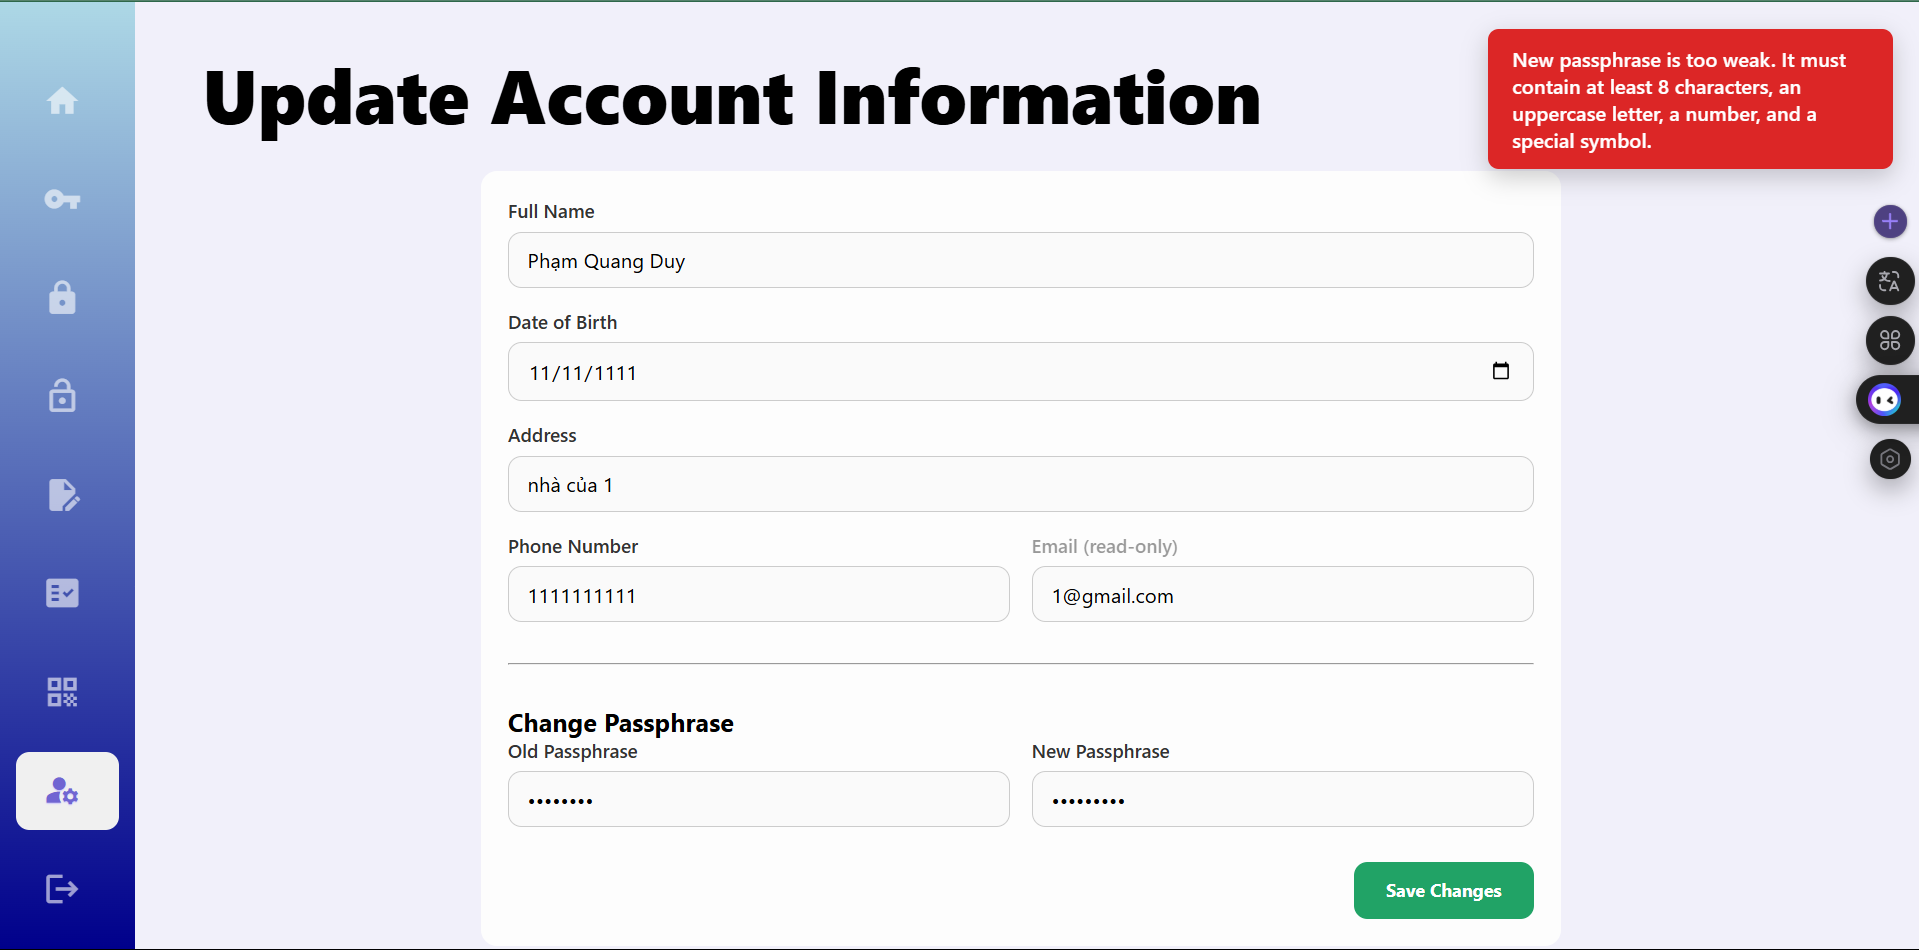
\includegraphics[width=0.85\textwidth]{img/5_update/5_update_fail_1.png}
        \caption{Thông báo lỗi khi kiểm tra đầu vào}
    \end{figure}

    \begin{figure}[H]
        \centering
        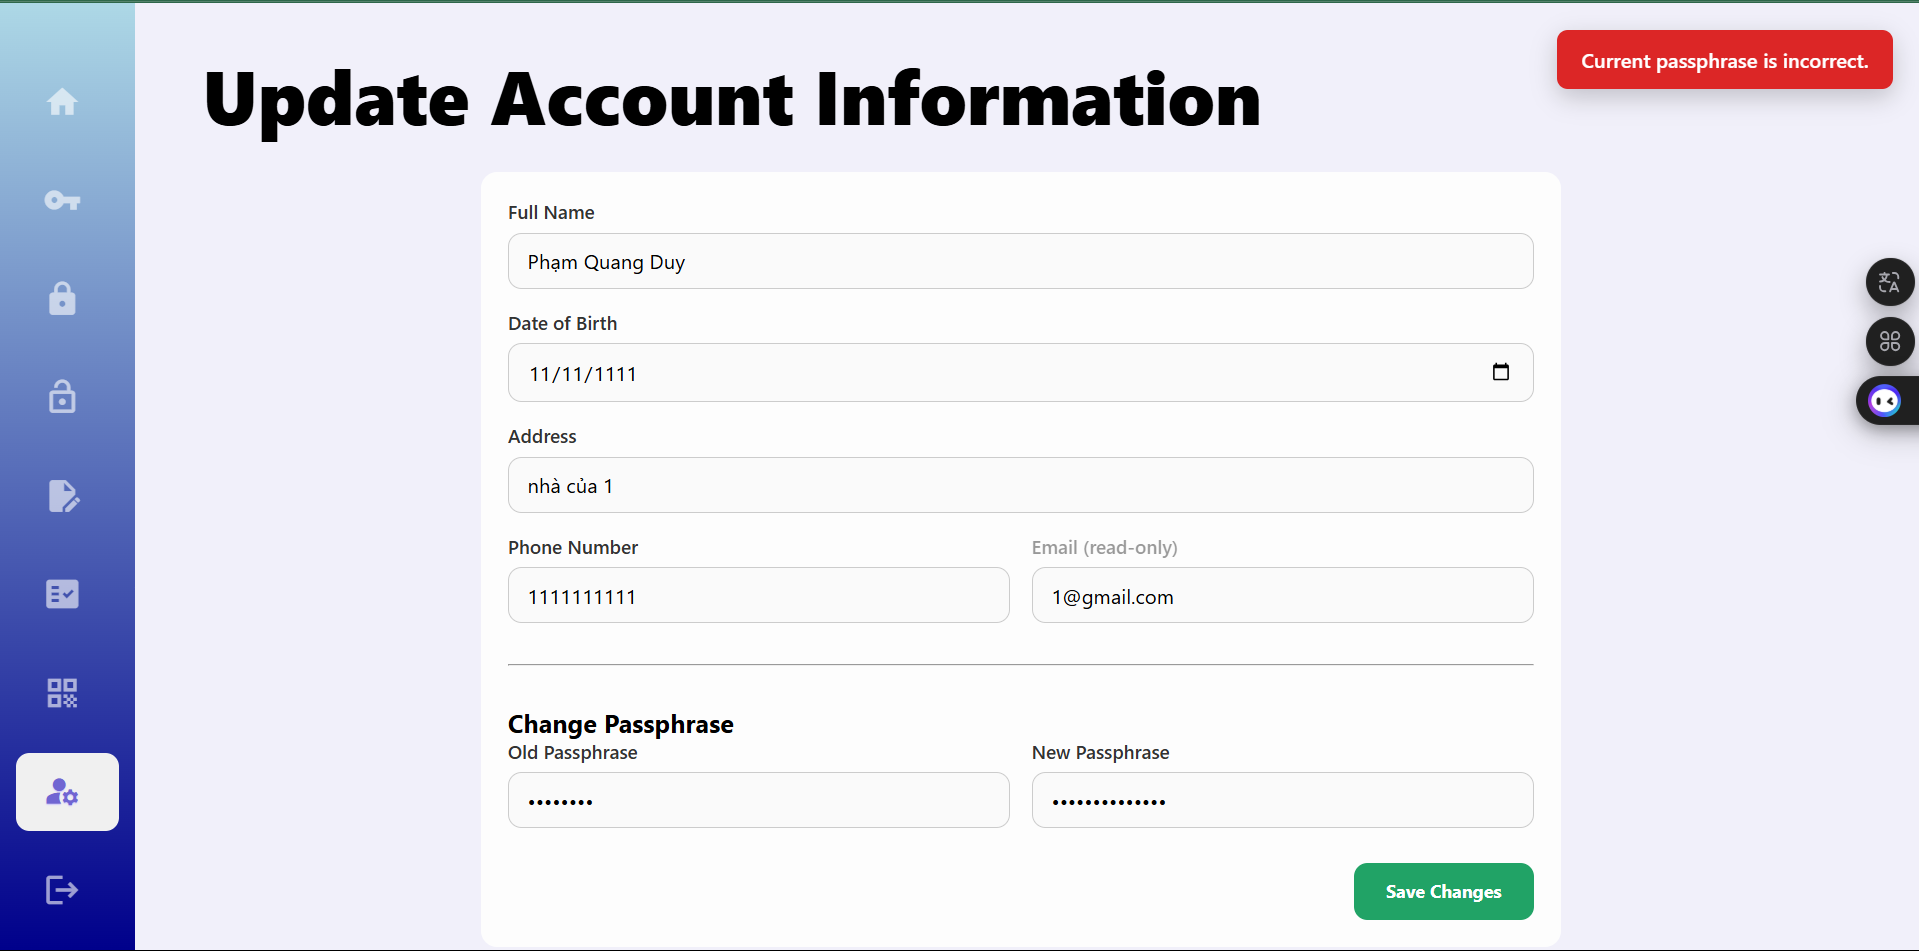
\includegraphics[width=0.85\textwidth]{img/5_update/5_update_fail_2.png}
        \caption{Thông báo lỗi khi kiểm tra đầu vào}
    \end{figure}

    \begin{figure}[H]
        \centering
        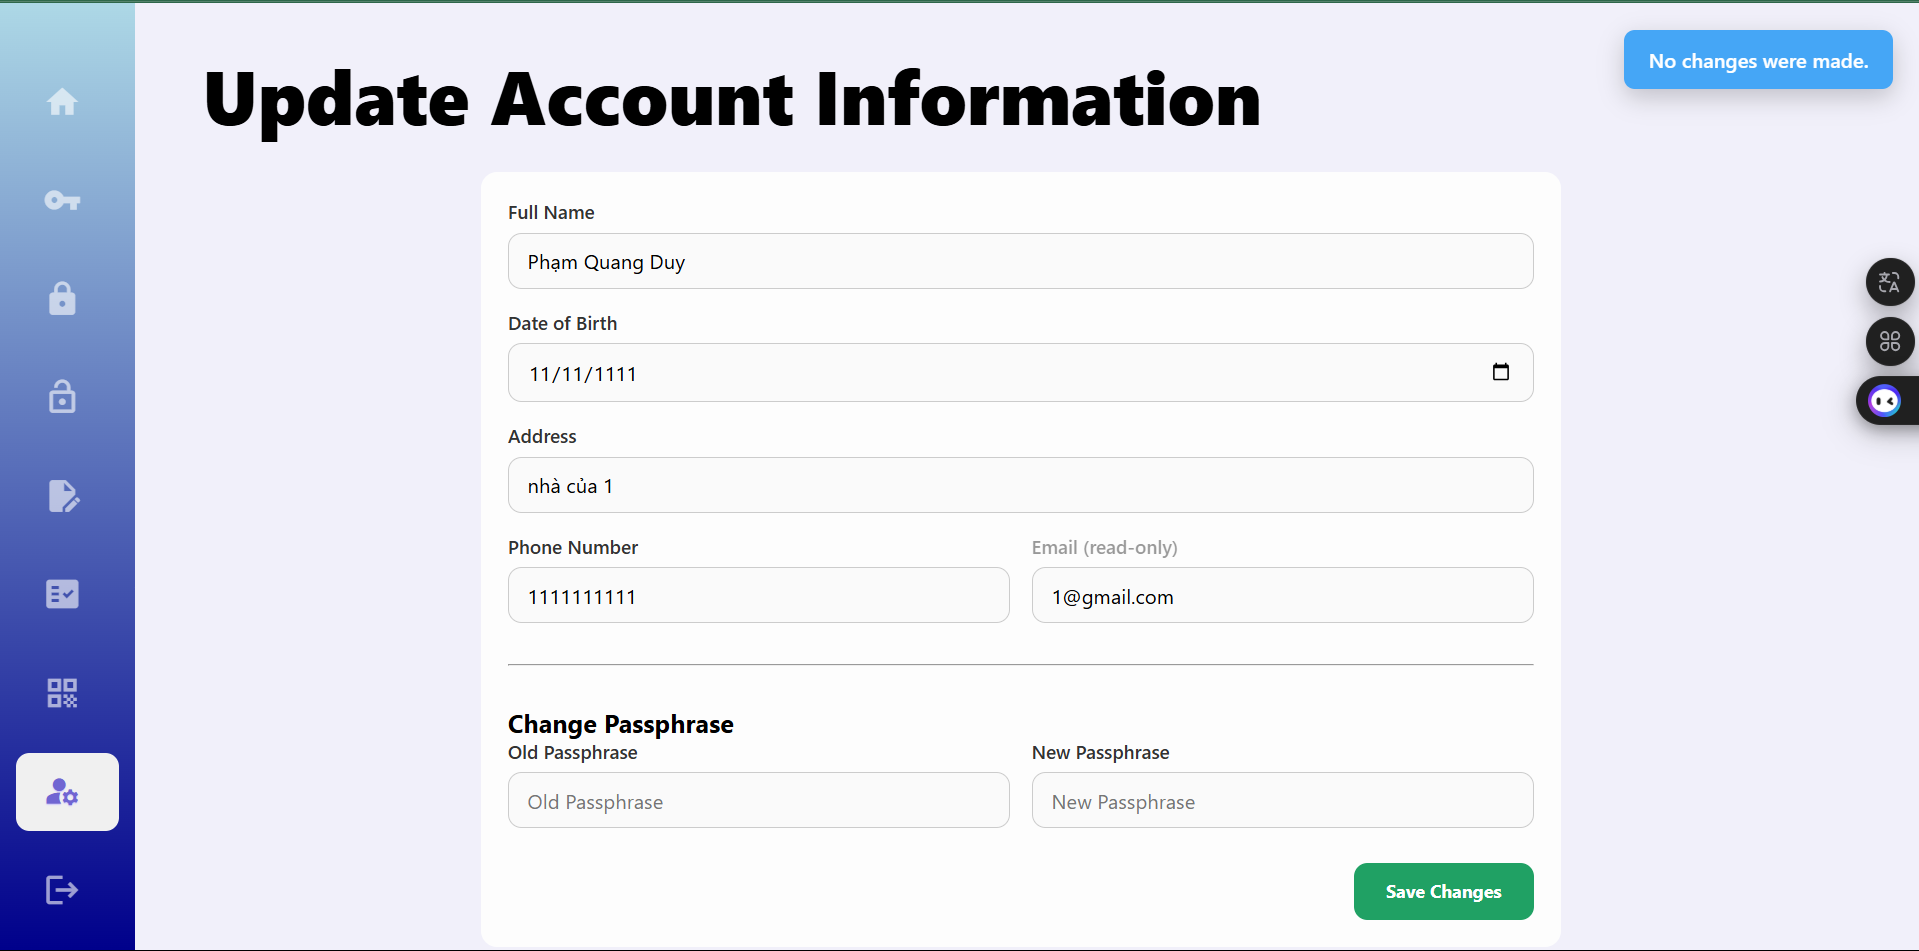
\includegraphics[width=0.85\textwidth]{img/5_update/5_update_no_changes.png}
        \caption{Thông báo khi không có thay đổi}
    \end{figure}
\end{description}

\newpage
\subsection{Mã hoá tập tin gửi người khác}
\subsubsection*{Mục tiêu}

\subsubsection*{Giao diện}

\subsubsection*{Quy trình thực hiện}

\subsubsection*{Chi tiết kỹ thuật và thư viện bảo mật}
\newpage
\subsection{Giải mã tập tin}
\subsubsection*{Mục tiêu}

\subsubsection*{Giao diện}

\subsubsection*{Quy trình thực hiện}

\subsubsection*{Chi tiết kỹ thuật và thư viện bảo mật}
\newpage
\subsection{Ký số tập tin}
\subsubsection*{Mục tiêu}

\subsubsection*{Giao diện}

\subsubsection*{Quy trình thực hiện}

\subsubsection*{Chi tiết kỹ thuật và thư viện bảo mật}
\newpage
\subsection{Xác minh chữ ký}
\subsubsection*{Mục tiêu}

\subsubsection*{Giao diện}

\subsubsection*{Quy trình thực hiện}

\subsubsection*{Chi tiết kỹ thuật và thư viện bảo mật}
\newpage
\subsection{Phân quyền tài khoản}
\subsubsection*{Mục tiêu}

\subsubsection*{Giao diện}

\subsubsection*{Quy trình thực hiện}

\subsubsection*{Chi tiết kỹ thuật và thư viện bảo mật}
\newpage
\subsection{Ghi log bảo mật}

\subsubsection*{Mục tiêu}
Chức năng ghi log bảo mật nhằm đảm bảo toàn bộ hành động của người dùng và các sự kiện nội bộ trong hệ thống đều được theo dõi, ghi nhận và lưu trữ dưới dạng thống nhất. Việc này phục vụ:
\begin{itemize}
    \item Truy vết các hành động quan trọng: đăng nhập, ký số, xác minh,...
    \item Giám sát lỗi bảo mật và cảnh báo bất thường.
    \item Làm bằng chứng trong điều tra sự cố hoặc kiểm toán.
\end{itemize}

\subsubsection*{Giao diện}
Giao diện tại trang \texttt{/admin\_dashboard} cung cấp:
\begin{itemize}
    \item Bảng hiển thị đầy đủ log: thời gian, mức độ (INFO, WARNING, ERROR), email người dùng, hành động, trạng thái và chi tiết.
    \item Tính năng tìm kiếm realtime và nút \texttt{Reload} để làm mới dữ liệu.
    \item Dữ liệu được render động thông qua fetch \texttt{X-Requested-With = XMLHttpRequest}.
\end{itemize}

\begin{figure}[H]
    \centering
    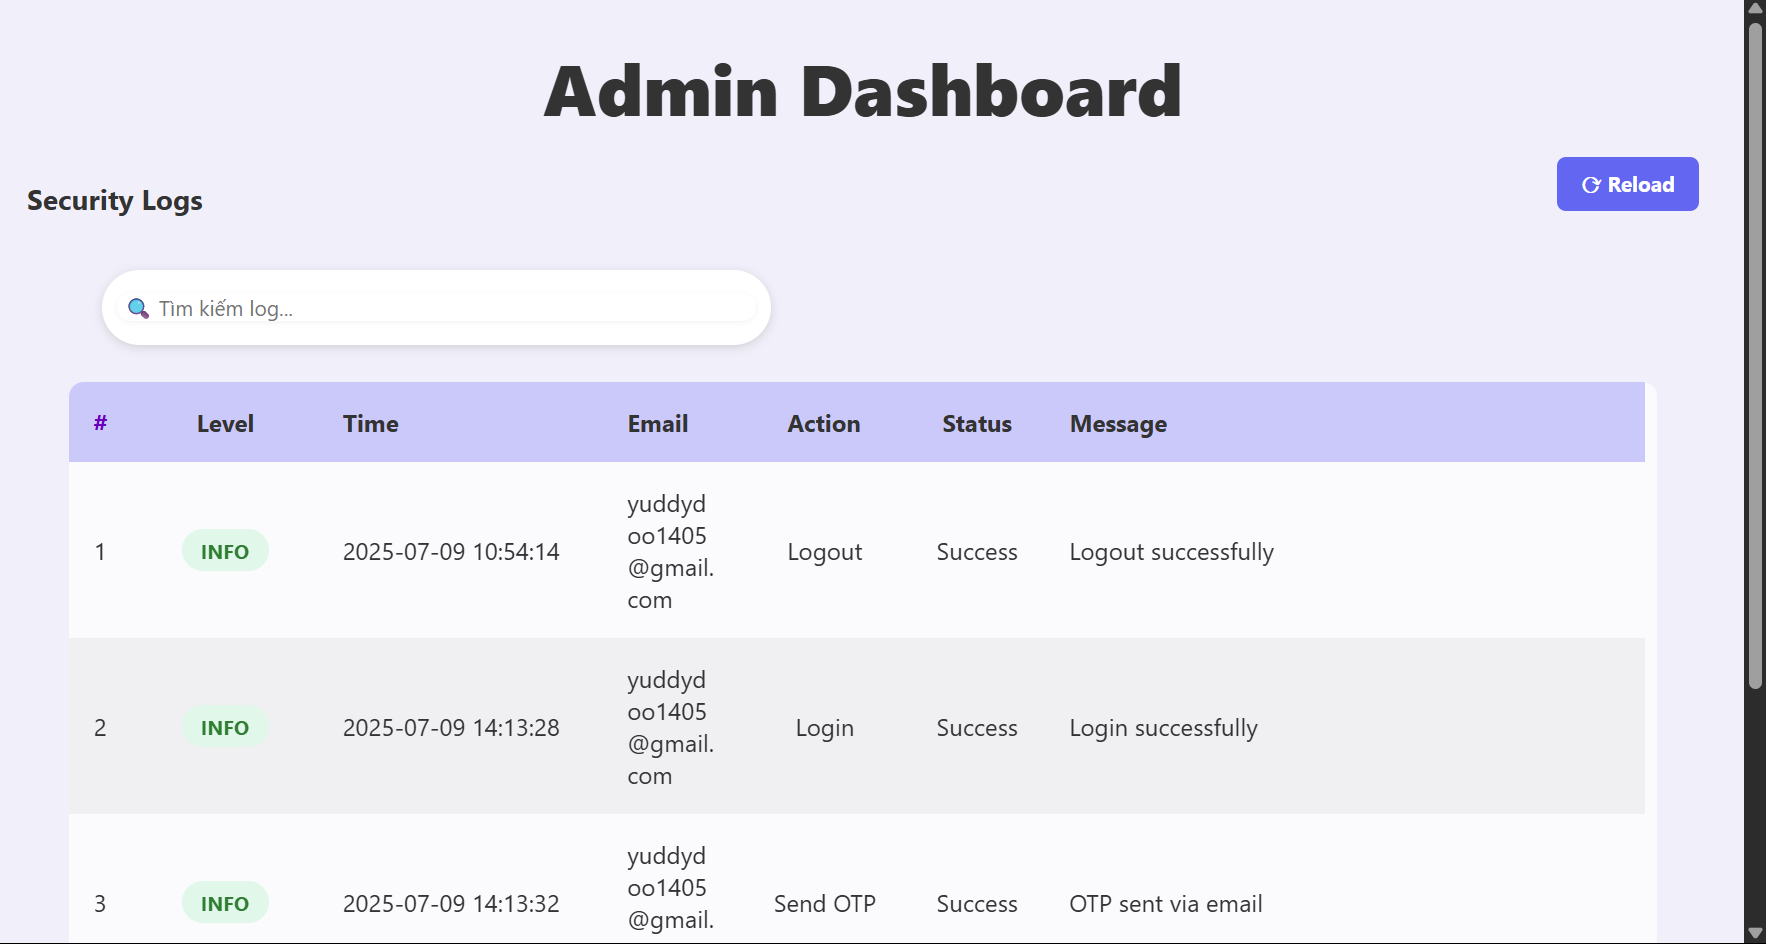
\includegraphics[width=0.85\textwidth]{img/11_logger/11_logger_table.png}
    \caption{Bảng log của admin}
\end{figure}

\subsubsection*{Quy trình thực hiện}
\begin{description}
    \item[\textbf{1. Người dùng thực hiện hành động}]
    Mỗi khi người dùng thao tác (ví dụ: đăng nhập, ký file, xác minh), hàm \texttt{log\_user\_action()} được gọi để ghi log với thông tin đầy đủ: email, hành động, trạng thái, chi tiết và mức độ severity.

    \begin{figure}[H]
        \centering
        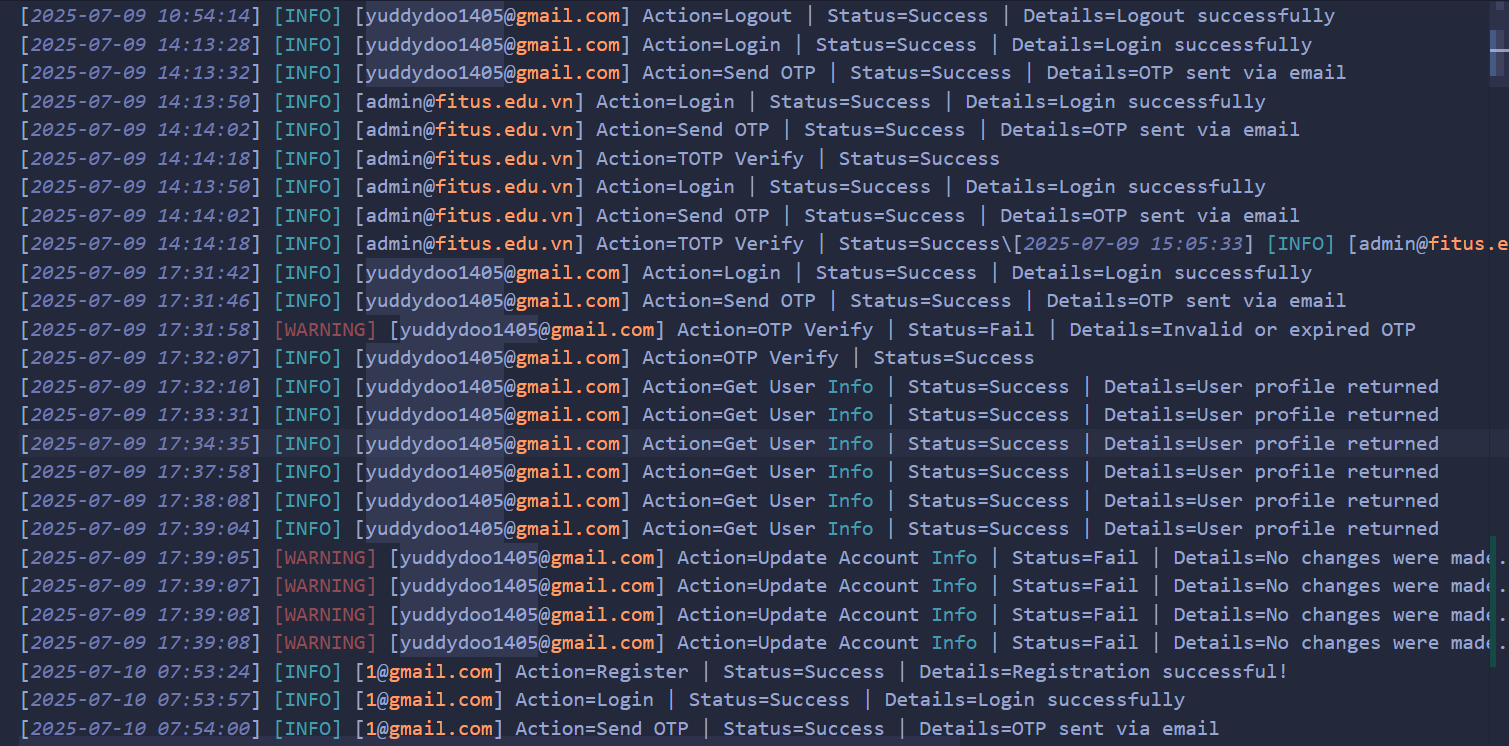
\includegraphics[width=0.85\textwidth]{img/11_logger/11_logger_file.png}
        \caption{Log cho người dùng - Routes}
    \end{figure}

    \item[\textbf{2. Hệ thống nội bộ phát sinh sự kiện}]
    Các module nội bộ (như mã hóa, xác minh chữ ký) có thể gọi \texttt{log\_internal\_event()} để ghi lại log kỹ thuật chi tiết.
    \begin{figure}[H]
        \centering
        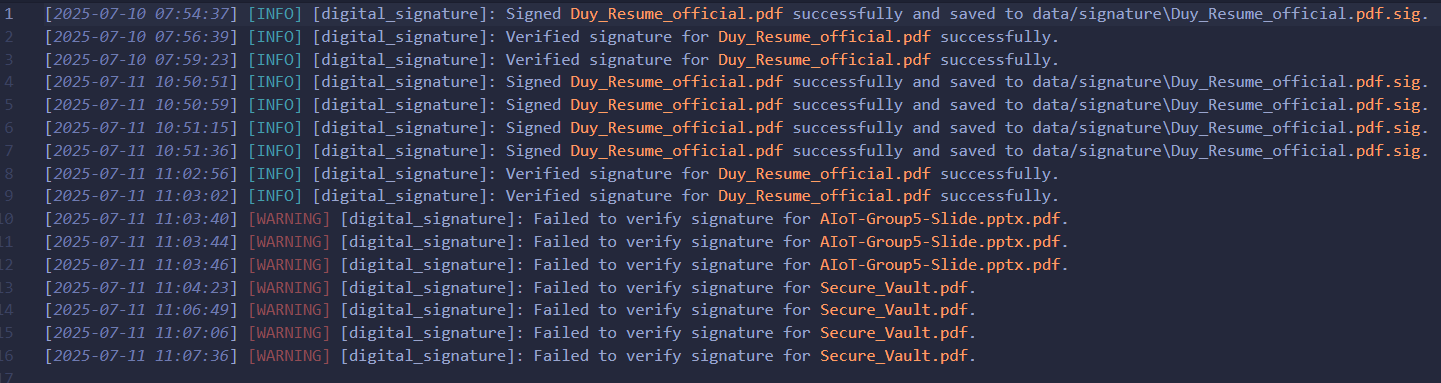
\includegraphics[width=0.85\textwidth]{img/11_logger/11_logger_debug.png}
        \caption{Log cho debug - Modules}
    \end{figure}

    \item[\textbf{3. Lưu vào file log}]
    Log người dùng và log nội bộ để debug sẽ được lưu vào các file riêng
    \begin{itemize}
        \item Log người dùng được ghi vào \texttt{log/security.log}
        \item Log module nội bộ được ghi vào \texttt{log/debug\_log.log}
    \end{itemize}

    \item[\textbf{4. Giao diện đọc log}]
    Khi người dùng truy cập trang \texttt{/admin\_dashboard}, Flask route đọc và phân tích nội dung từ file log, chuyển thành danh sách JSON và hiển thị trên giao diện.
\end{description}

\subsubsection*{Chi tiết kỹ thuật và thư viện bảo mật}
\begin{description}

    \item[\textbf{1. Hàm log người dùng}]
    \texttt{log\_user\_action(email, action, status, details, level)} ghi log theo format thống nhất:
    \begin{itemize}
        \item Ví dụ log: \texttt{[2025-07-09 10:15:23] [INFO] [user@example.com] Action=Sign File | Status=Success | Details=file=report.pdf}
        \item Sử dụng thư viện chuẩn \texttt{logging}, ghi vào \texttt{log/security.log}
    \end{itemize}

    \item[\textbf{2. Log nội bộ hệ thống}]
    \texttt{log\_internal\_event(module, message, level)} dùng cho debug các module như crypto, xác minh,...
    \begin{itemize}
        \item Ví dụ: \texttt{[crypto]: Signature verified successfully.}
        \item Ghi vào \texttt{log/debug\_log.log} với format chi tiết hơn để phục vụ debug.
    \end{itemize}

    \item[\textbf{3. Route hiển thị log}]
    Route \texttt{/log\_security} thực hiện:
    \begin{itemize}
        \item Đọc file \texttt{log/security.log}, tách thành các trường: \texttt{timestamp, level, user, action, status, details}
        \item Trả về \texttt{JSON} nếu là AJAX, hoặc render giao diện nếu là truy cập thường
    \end{itemize}

    \item[\textbf{4. Mức độ log hỗ trợ}]
    \begin{itemize}
        \item \texttt{INFO} – hành động thành công hoặc hợp lệ
        \item \texttt{WARNING} – thao tác sai, lỗi thường gặp
        \item \texttt{ERROR} – lỗi hệ thống hoặc dữ liệu bất thường
        \item \texttt{DEBUG} – dành cho log kỹ thuật nội bộ (chỉ module log mới dùng)
    \end{itemize}

    \item[\textbf{5. Định dạng và chuẩn hóa log}]
    Mọi log đều tuân thủ format:
    \begin{quote}
        \texttt{[timestamp] [LEVEL] [email] Action=... | Status=... | Details=...}
    \end{quote}
    Điều này giúp dễ dàng phân tích bằng tool, lọc log, và hỗ trợ audit.

\end{description}

\newpage
\subsection{Chia nhỏ tập tin lớn}
\subsubsection*{Mục tiêu}

\subsubsection*{Giao diện}

\subsubsection*{Quy trình thực hiện}

\subsubsection*{Chi tiết kỹ thuật và thư viện bảo mật}
\newpage
\subsection{Kiểm tra trạng thái khoá}
\subsubsection*{Mục tiêu}

\subsubsection*{Giao diện}

\subsubsection*{Quy trình thực hiện}

\subsubsection*{Chi tiết kỹ thuật và thư viện bảo mật}
\newpage
\subsection{Tìm kiếm public key}

\subsubsection*{Mục tiêu}
Chức năng này cho phép người dùng tìm kiếm trong danh sách các public key đã lưu (của các liên hệ khác). Việc quản lý và tìm nhanh public key giúp người dùng dễ dàng sử dụng trong quá trình mã hóa, xác minh chữ ký, và chia sẻ an toàn.

\subsubsection*{Giao diện}
Giao diện tại tab \texttt{Owned Public Keys} trong dashboard bao gồm:
\begin{itemize}
    \item Bảng hiển thị danh sách các public key đã lưu: tên người gửi, email, timestamp và public key.
    \item Ô tìm kiếm theo email hoặc public key (tìm mờ, không phân biệt hoa thường).
    \item Dữ liệu được lấy động từ API \texttt{/owned\_keys}.
\end{itemize}

\begin{figure}[H]
    \centering
    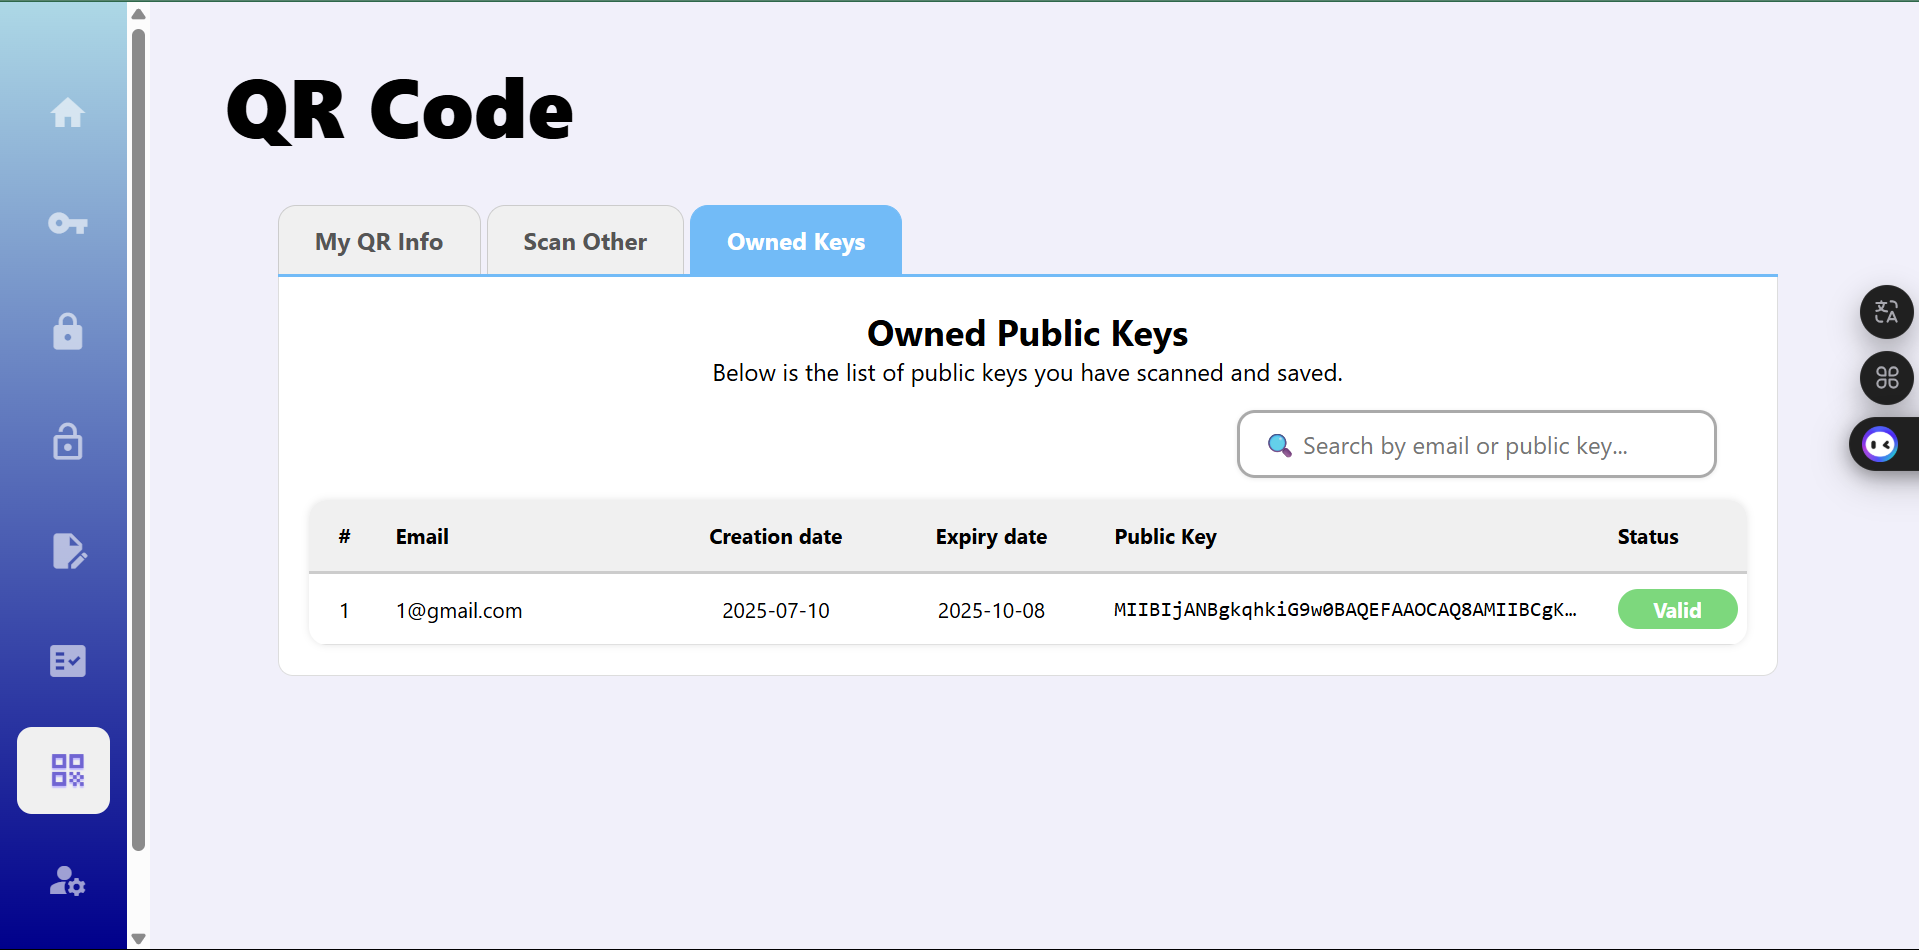
\includegraphics[width=0.85\textwidth]{img/14_pubkey/14_pubkey_ui.png}
    \caption{Danh sách contact - public key đã lưu}
\end{figure}

\subsubsection*{Quy trình thực hiện}
\begin{description}
    \item[\textbf{1. Truy cập tab Owned Keys}]
    Người dùng đăng nhập và truy cập trang dashboard → phần "Owned Public Keys" sẽ gửi request GET đến API \texttt{/owned\_keys}.

    \item[\textbf{2. API lấy dữ liệu}]
    Flask route \texttt{/owned\_keys} thực hiện:
    \begin{itemize}
        \item Kiểm tra phiên đăng nhập.
        \item Đọc file \texttt{contact\_public\_key.json} theo thư mục cá nhân người dùng.
        \item Chuyển danh sách public key về dạng JSON và trả về frontend.
    \end{itemize}

    \item[\textbf{3. Hiển thị và tìm kiếm}]
    \begin{itemize}
        \item JavaScript tạo bảng dữ liệu từ kết quả JSON trả về.
        \item Khi người dùng gõ từ khóa vào ô tìm kiếm, hàm \texttt{filterPublicKeys()} lọc các hàng phù hợp theo email hoặc chuỗi public key.
    \end{itemize}
\end{description}

\subsubsection*{Chi tiết kỹ thuật và thư viện bảo mật}
\begin{description}

    \item[\textbf{1. Cấu trúc lưu public key}]
    \begin{itemize}
        \item Mỗi người dùng có một file riêng: \texttt{<user\_email>/contact\_public\_key.json}
        \item Dạng JSON: \texttt{\{"abc@example.com": \{"name": ..., "public\_key\_pem": ...\}\}}
    \end{itemize}

    \item[\textbf{2. API trả dữ liệu public key}]
    \texttt{/owned\_keys} là route GET:
    \begin{itemize}
        \item Nếu chưa đăng nhập → trả lỗi \texttt{401 Unauthorized}.
        \item Nếu file danh bạ không tồn tại → trả danh sách rỗng.
        \item Ghi log trạng thái truy vấn bằng \texttt{log\_user\_action(...)} với số lượng public key tìm được.
    \end{itemize}

    \item[\textbf{3. Tìm kiếm phía client}]
    \begin{itemize}
        \item Hàm \texttt{filterPublicKeys()} lọc dữ liệu theo từ khóa không phân biệt hoa thường.
        \item Kiểm tra xem từ khóa xuất hiện trong email hoặc chuỗi public key PEM.
        \item Lọc trực tiếp trên DOM → không gọi lại API khi tìm kiếm.
    \end{itemize}

    \item[\textbf{4. Hiển thị QR code public key}]
    Hệ thống hỗ trợ hiển thị mã QR của public key khi người dùng click vào một contact cụ thể trong bảng danh sách. Điều này giúp việc chia sẻ public key giữa người dùng dễ dàng và nhanh chóng hơn (qua quét mã bằng điện thoại, Google Authenticator,...).

    \begin{itemize}
        \item Giao diện sử dụng sự kiện \texttt{onClick} hoặc nút \texttt{View QR} gắn với mỗi hàng trong bảng.
        \item Khi người dùng bấm chọn, mã public key PEM tương ứng sẽ được gửi đến route \texttt{/utils/generate\_qr} (hoặc sinh trực tiếp frontend).
        \item QR code được sinh từ chuỗi PEM hoặc JSON chứa các thông tin liên hệ và khóa công khai.
        \item Kết quả được hiển thị trong một modal hoặc khung bên cạnh dòng đã chọn.
        \item Mã QR cho phép người khác dễ dàng quét để lưu lại public key → hỗ trợ xác thực và mã hóa an toàn.
    \end{itemize}

    \begin{figure}[H]
        \centering
        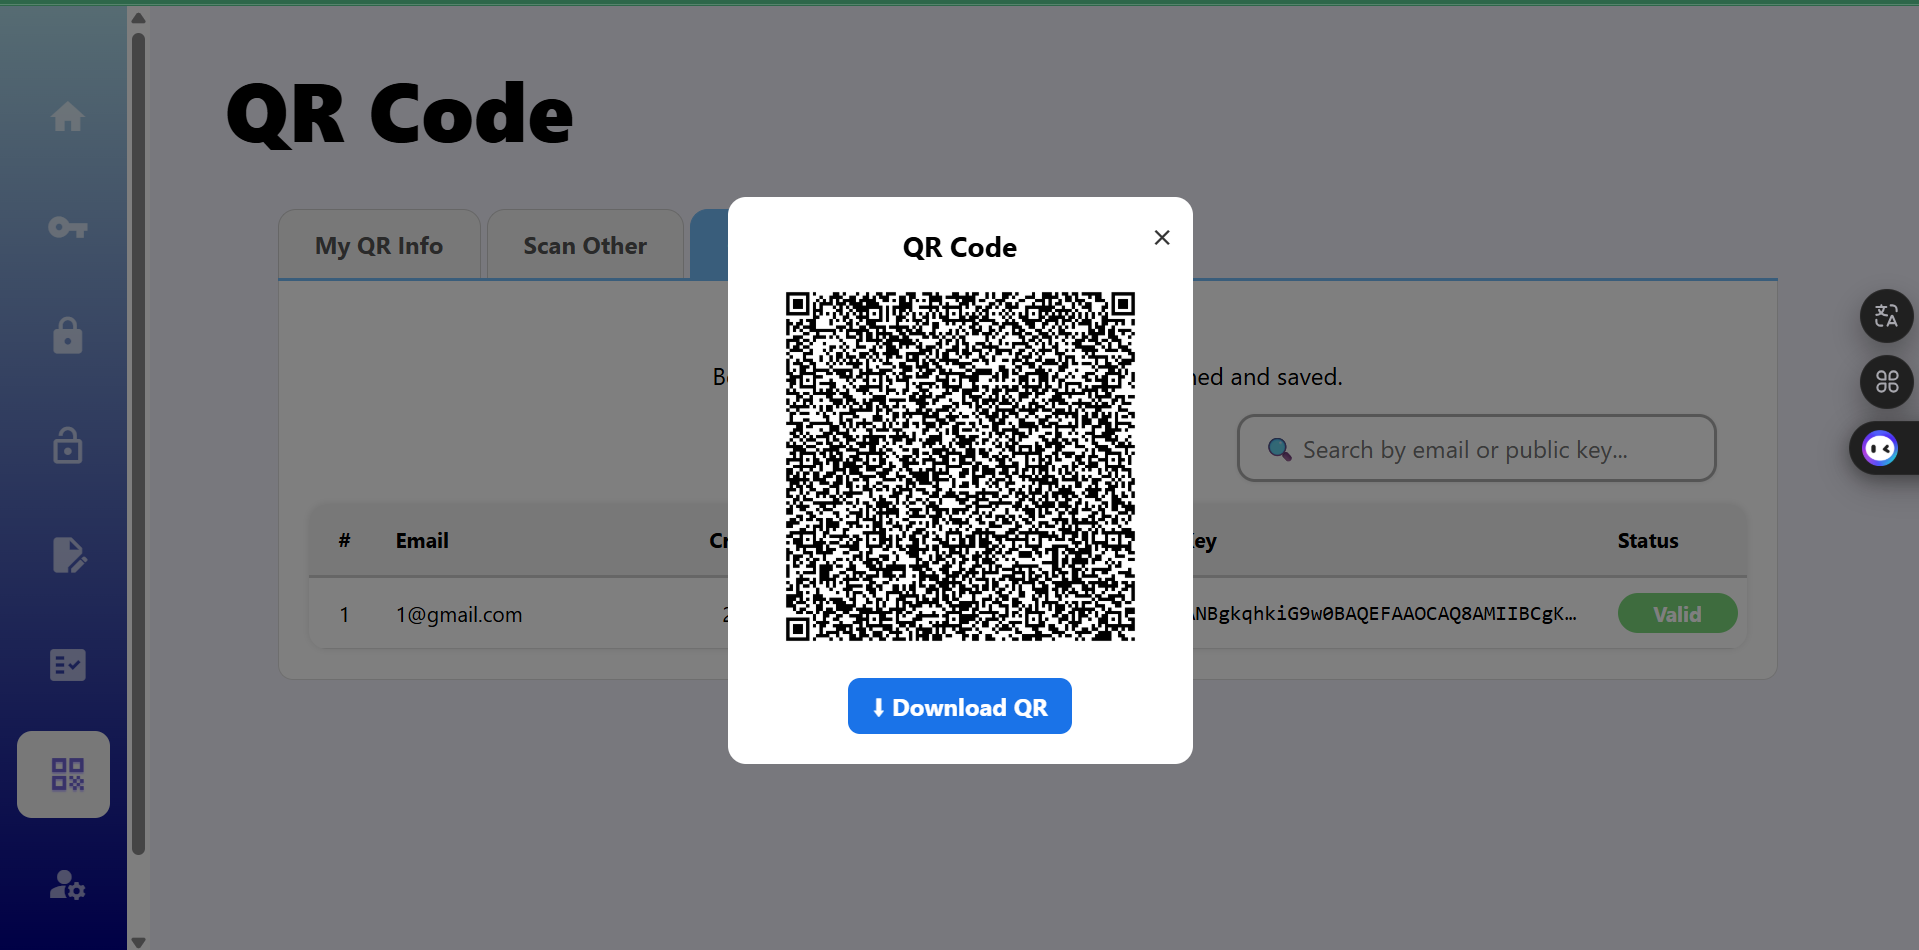
\includegraphics[width=0.85\textwidth]{img/14_pubkey/14_pubkey_qr.png}
        \caption{Pop-up QR của contact đã lưu}
    \end{figure}

    \item[\textbf{5. Bảo mật truy cập}]
    Chỉ người dùng đã đăng nhập mới được phép truy vấn danh sách public key đã lưu.
    \begin{itemize}
        \item File JSON được lưu riêng trong thư mục người dùng → cô lập dữ liệu từng tài khoản.
    \end{itemize}

\end{description}

\newpage
\subsection{Giới hạn đăng nhập}
\subsubsection*{Mục tiêu}

\subsubsection*{Giao diện}

\subsubsection*{Quy trình thực hiện}

\subsubsection*{Chi tiết kỹ thuật và thư viện bảo mật}
\newpage
\subsection{Tùy chọn định dạng lưu file}
\subsubsection*{Mục tiêu}

\subsubsection*{Giao diện}

\subsubsection*{Quy trình thực hiện}

\subsubsection*{Chi tiết kỹ thuật và thư viện bảo mật}
\newpage
\subsection{Khôi phục tài khoản}

\subsubsection*{Mục tiêu}
Chức năng khôi phục tài khoản cho phép người dùng đặt lại mật khẩu (passphrase) khi không còn nhớ mật khẩu cũ. Khác với đặt lại mật khẩu thông thường, hệ thống vẫn đảm bảo khôi phục được private key đã mã hóa trước đó – nhờ sử dụng một \textbf{recovery code} (AES key phụ) đã được lưu trữ an toàn từ khi đăng ký.

\subsubsection*{Giao diện}
Giao diện khôi phục gồm 2 bước:
\begin{itemize}
    \item \textbf{Bước 1:} Người dùng nhập email và recovery code để xác minh quyền sở hữu tài khoản.
    \begin{figure}[H]
        \centering
        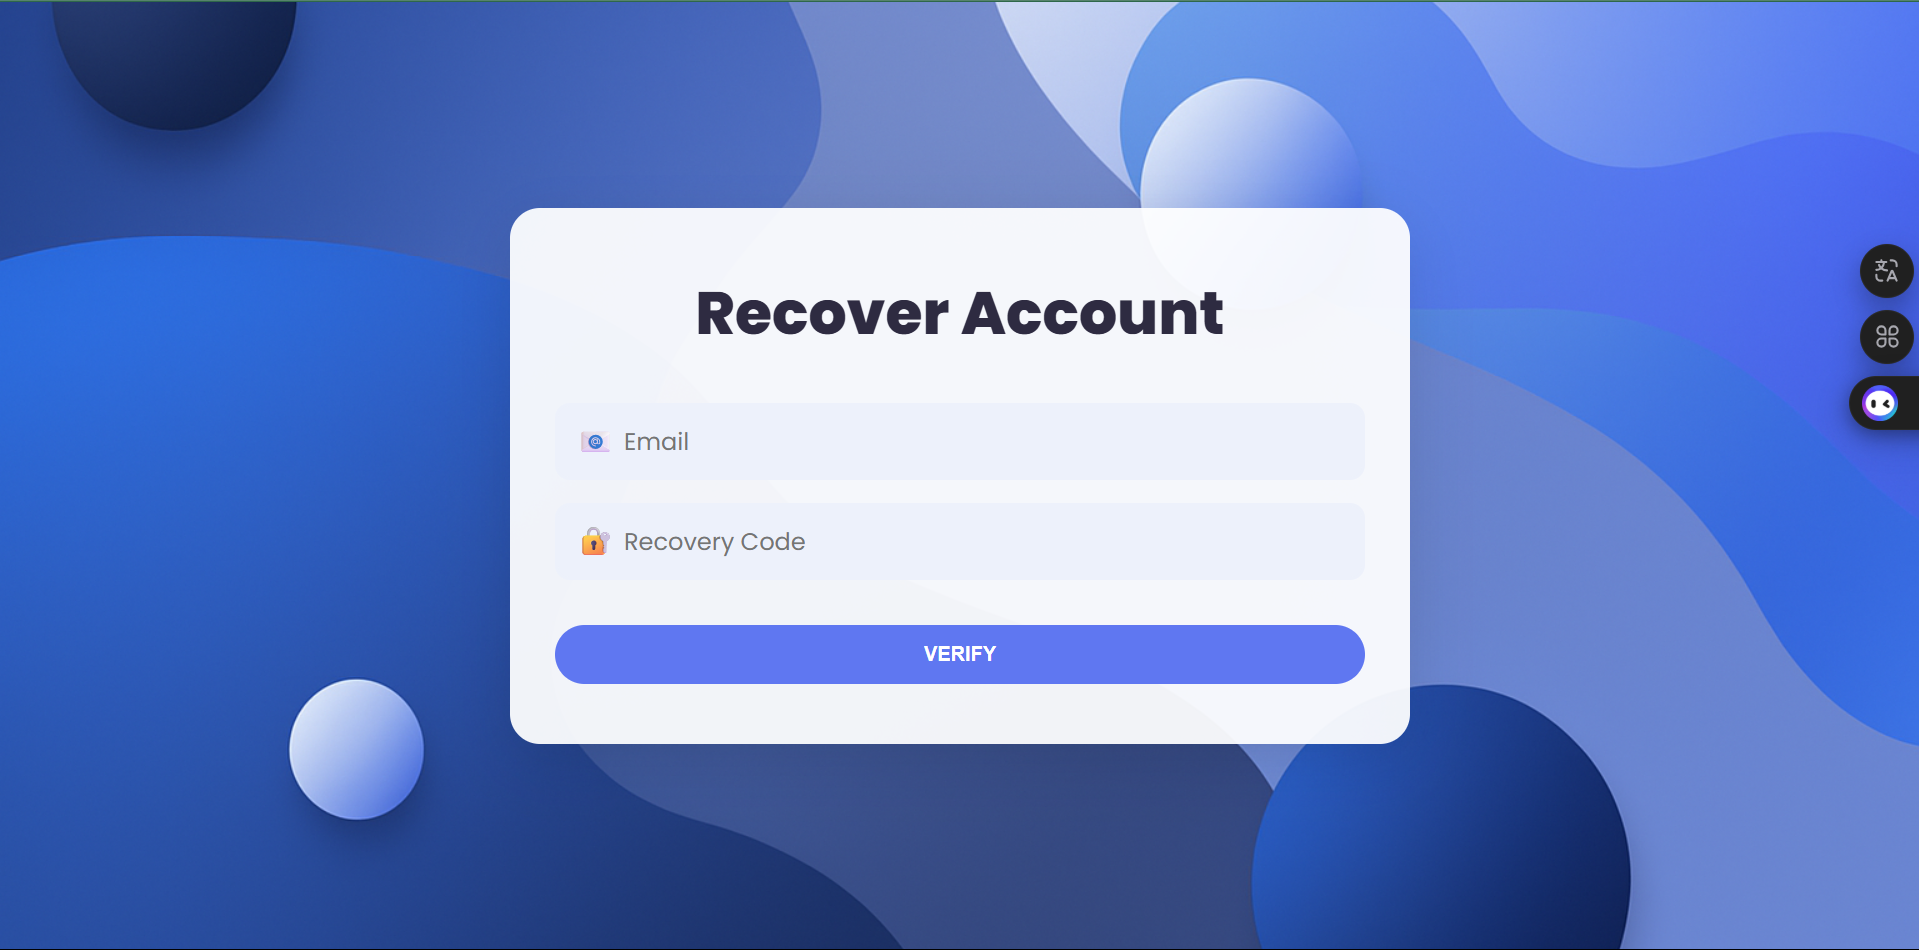
\includegraphics[width=0.85\textwidth]{img/17_recover/17_recover_recovery_code.png}
        \caption{Nhập mã khôi phục}
    \end{figure}

    \item \textbf{Bước 2:} Nếu thành công, hệ thống cho phép nhập mật khẩu mới (passphrase), sau đó sẽ mã hóa lại khóa riêng và recovery key.
    \begin{figure}[H]
        \centering
        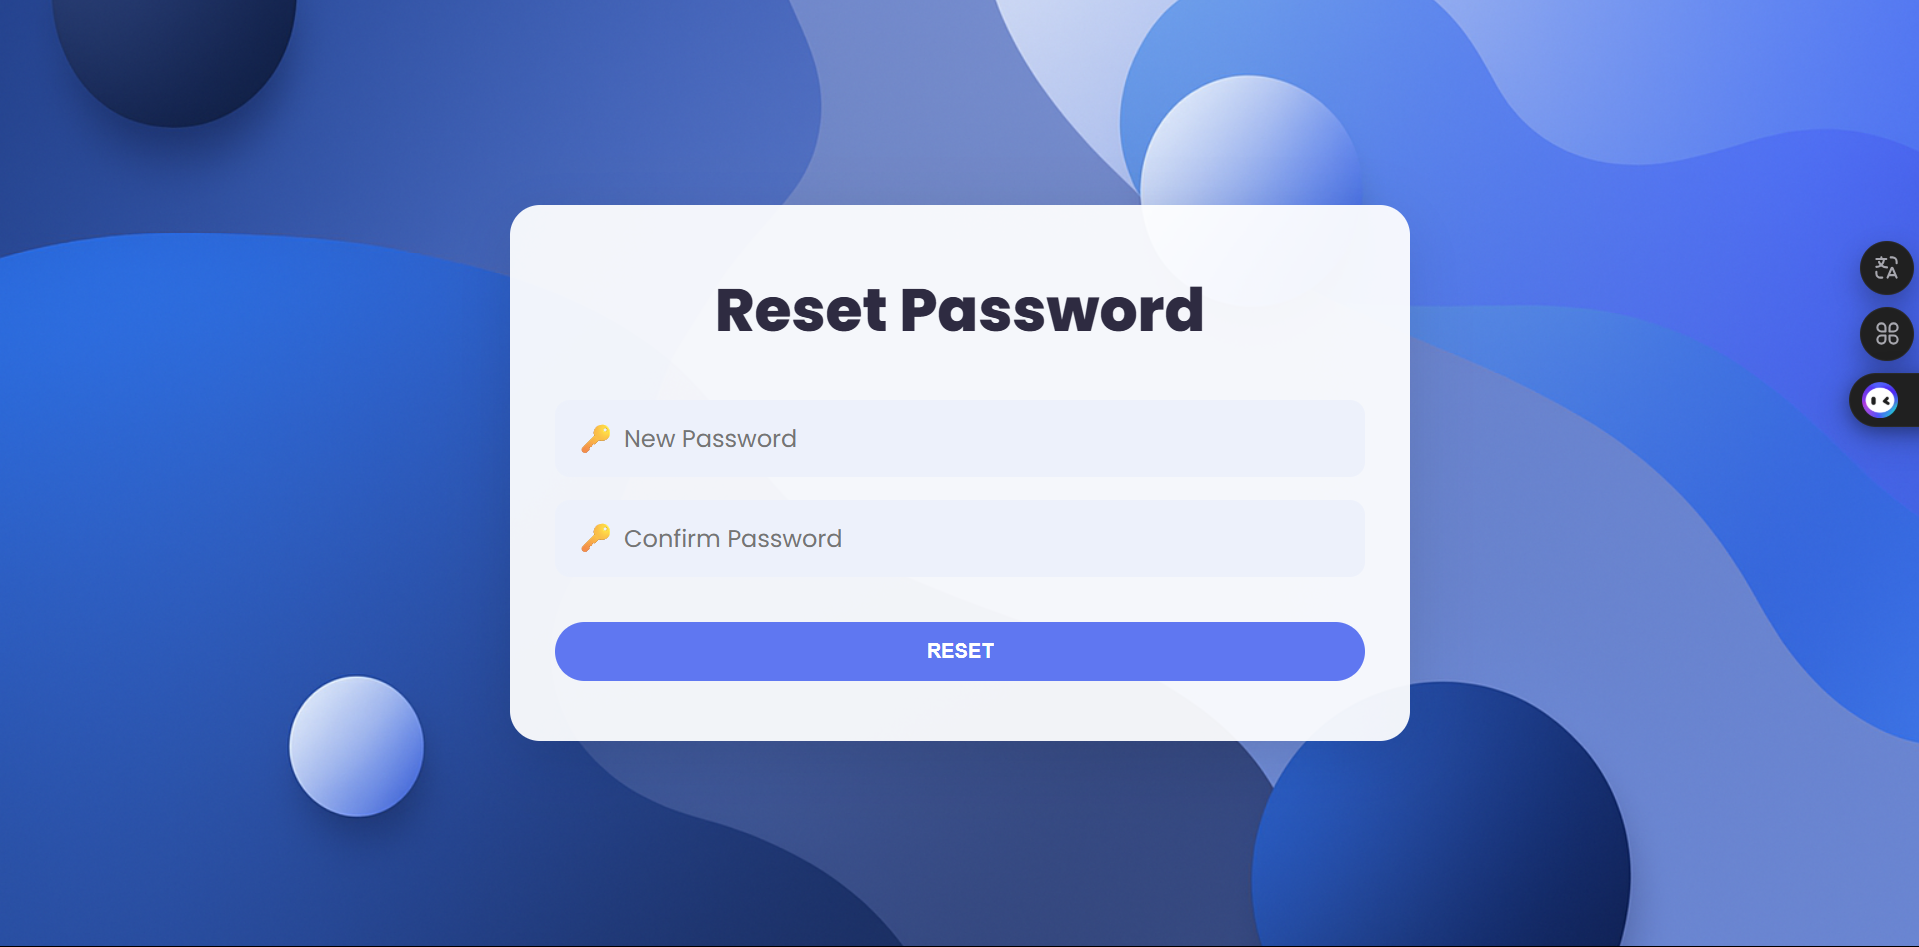
\includegraphics[width=0.85\textwidth]{img/17_recover/17_recovery_pw.png}
        \caption{Nhập mật khẩu mới}
    \end{figure}
\end{itemize}

\subsubsection*{Quy trình thực hiện}
\begin{description}

    \item[\textbf{Bước 1 - Xác minh recovery code}]
    \begin{itemize}
        \item Người dùng nhập recovery code → hệ thống derive AES key từ recovery code đó.
        \item Dùng AES key này để giải mã file \texttt{key\_recovery} chứa private key hiện tại.
        \item Nếu giải mã thành công → recovery code hợp lệ.
    \end{itemize}

    \item[\textbf{Bước 2 - Nhập mật khẩu mới}]
    \begin{itemize}
        \item Người dùng nhập passphrase mới.
        \item Hệ thống mã hóa lại private key hiện tại bằng AES key derive từ passphrase mới.
        \item Đồng thời, mã hóa lại recovery code bằng AES key derive từ passphrase mới → lưu vào cột \texttt{encrypted\_recovery\_code} trong database.
    \end{itemize}

    \item[\textbf{Bước 3 - Cập nhật cơ sở dữ liệu}]
    \begin{itemize}
        \item Hash passphrase mới và cập nhật vào cột \texttt{hashed\_passphrase}.
        \item Ghi log hành động khôi phục với trạng thái thành công hoặc thất bại.
    \end{itemize}
\end{description}

\subsubsection*{Chi tiết kỹ thuật và thư viện bảo mật}
\begin{description}

    \item[\textbf{1. Recovery code}]
    Recovery code là một chuỗi ngẫu nhiên sinh ra khi đăng ký, dùng để derive AES key tạm thời cho mục đích khôi phục khóa.
    \begin{itemize}
        \item Được dùng để giải mã private key hiện tại khi muốn reset password. 
        \item Được mã hóa bằng AES key derive từ passphrase và lưu dưới database.
    \end{itemize}

    \item[\textbf{2. Kiểm tra tính hợp lệ của recovery code}]
    \begin{itemize}
        \item Dùng recovery code derive AES key: \texttt{derive\_aes\_key(recovery\_code)}.
        \item Giải mã file \texttt{key\_recovery} (chứa private key mã hóa) bằng AES key này.
        \item Nếu giải mã được → xác minh thành công.
    \end{itemize}

    \item[\textbf{3. Đặt lại mật khẩu và mã hóa lại dữ liệu}]
    \begin{itemize}
        \item Derive AES key từ passphrase mới.
        \item Mã hóa lại private key bằng AES key mới.
        \item Mã hóa recovery code bằng AES key mới và lưu vào \texttt{encrypted\_recovery\_code}.
        \item Hash passphrase mới với salt → cập nhật vào bảng \texttt{users}.
    \end{itemize}

    \item[\textbf{4. Xử lý lỗi và báo lỗi chi tiết}]
    Hệ thống đảm bảo mọi lỗi trong quá trình khôi phục tài khoản đều được phát hiện, phản hồi rõ ràng cho người dùng, đồng thời ghi log bảo mật để hỗ trợ điều tra.

    \begin{itemize}
        \item \textbf{Thiếu email hoặc recovery code:}
        \begin{itemize}
            \item Nếu không gửi đủ thông tin đầu vào → trả lỗi \texttt{400} với thông báo: \texttt{"Missing recovery information"}.
        \end{itemize}

        \item \textbf{Recovery code không hợp lệ:}
        \begin{itemize}
            \item Nếu recovery code không trùng khớp hoặc giải mã private key thất bại → trả lỗi \texttt{400}, thông báo: \texttt{"Invalid recovery code"}.
            \item Lỗi này thường do nhập sai hoặc đã đổi passphrase trước đó mà chưa cập nhật lại recovery key.
        \end{itemize}

        \item \textbf{Mật khẩu mới không hợp lệ:}
        \begin{itemize}
            \item Nếu passphrase mới không đủ mạnh (dưới 8 ký tự, không có ký tự đặc biệt, chữ hoa, số) → từ chối và trả thông báo cụ thể.
        \end{itemize}

        \item \textbf{Lỗi mã hóa lại private key hoặc recovery key:}
        \begin{itemize}
            \item Nếu trong quá trình mã hóa lại private key bằng passphrase mới xảy ra lỗi → rollback thao tác DB và trả về lỗi \texttt{"Re-encrypt RSA failed"}.
            \item Nếu mã hóa lại recovery key lỗi → báo lỗi \texttt{"Failed to encrypt recovery key"} và không cập nhật thông tin.
        \end{itemize}

        \item \textbf{Lỗi cập nhật CSDL:}
        \begin{itemize}
            \item Nếu xảy ra lỗi khi cập nhật passphrase hoặc encrypted recovery key trong database → trả lỗi \texttt{"Database error"} và log ở mức \texttt{error}.
        \end{itemize}

        \item \textbf{Log đầy đủ:}
        \begin{itemize}
            \item Tất cả lỗi đều được ghi lại bằng \texttt{log\_user\_action(...)} với trạng thái \texttt{"Fail"} và nội dung chi tiết.
            \item Các lỗi hệ thống (mã hóa thất bại, không đọc được recovery file, lỗi DB) được log với \texttt{level = "error"}.
        \end{itemize}
    \end{itemize}


\end{description}


\newpage
\section{Kiểm thử ứng dụng}
Tất cả hình ảnh kết quả kiểm thử được cập nhật đầy đủ trong \href{https://drive.google.com/drive/folders/1xRaJ4qGiTHa1X5nbth9Pzn4xKZmUR-6U?usp=sharing}{drive sau}
\subsection*{6.1 Đăng ký tài khoản người dùng (/signup)}
\begin{table}[H]
\centering
\begin{tabular}{|>{\centering\arraybackslash}p{4.3cm}|>{\arraybackslash}p{5cm}|>{\centering\arraybackslash}p{7.5cm}|}
\hline
\textbf{Mô tả kiểm thử} & 
\multicolumn{1}{>{\centering\arraybackslash}p{5cm}|}{\textbf{Input}} & 
\textbf{Kết quả mong đợi} \\ \hline
Đăng ký thành công & Email hợp lệ, Passphrase mạnh, các trường đầy đủ
 & Thông báo "Registration successful", pop-up \codefile{recovery\_code} \\ \hline
Email sai định dạng & \codefile{abc@.com} & Báo lỗi "Invalid email format" \\ \hline
Passphrase yếu & abc12345 & Báo lỗi "Passphrase too weak" \\ \hline
Trùng email đã đăng ký & Email đã có trong DB & Báo lỗi “Account already exists" \\ \hline
XSS/SQL injection & \codefile{<script>}, \codefile{" OR "1"="1} & Bị sanitize, không lỗi hệ thống \\ \hline
\end{tabular}
\end{table}

\subsection*{6.2 Đăng nhập và xác thực đa yếu tố (/login → /verify)}
\begin{table}[H]
\centering
\begin{tabular}{|>{\centering\arraybackslash}p{4.3cm}|>{\arraybackslash}p{5cm}|>{\centering\arraybackslash}p{7.5cm}|}
\hline
\textbf{Mô tả kiểm thử} &
\multicolumn{1}{>{\centering\arraybackslash}p{5cm}|}{\textbf{Input}} & 
\textbf{Kết quả mong đợi} \\ \hline
Đăng nhập đúng pass → chờ xác thực OTP & Email và passphrase đúng & Chuyển hướng tới trang \codefile{/verify} để xác thực OTP hoặc TOTP \\ \hline
Sai pass < 5 lần & Email đúng, passphrase sai & Báo lỗi “Wrong email or password” và tăng \codefile{failed\_attempts} \\ \hline
Sai pass ≥ 5 lần & Nhập sai liên tiếp 5 lần & Khóa tài khoản 5 phút, thông báo thời gian chờ \\ \hline
OTP hợp lệ trong thời gian & Mã OTP 6 chữ số từ email (trong vòng 5 phút) & Xác thực thành công, chuyển đến \codefile{/dashboard} hoặc \codefile{/admin\_dashboard} \\ \hline
OTP sai hoặc hết hạn & Mã OTP sai hoặc quá hạn 5 phút & Báo lỗi “Invalid or expired OTP” \\ \hline
TOTP đúng từ Google Authenticator & Mã 6 chữ số từ ứng dụng & Xác thực thành công, chuyển trang chính \\ \hline
TOTP sai & Nhập sai mã TOTP & Báo lỗi “Invalid TOTP code” \\ \hline
\end{tabular}
\end{table}

\subsection*{6.3 Quản lý khóa RSA cá nhân (/manage\_keys)}
\begin{table}[H]
\centering
\begin{tabular}{|>{\centering\arraybackslash}p{4.3cm}|>{\arraybackslash}p{5cm}|>{\centering\arraybackslash}p{7.5cm}|}
\hline
\textbf{Mô tả kiểm thử} & 
\multicolumn{1}{>{\centering\arraybackslash}p{5cm}|}{\textbf{Input}} & 
\textbf{Kết quả mong đợi} \\ \hline
Tạo cặp khóa thành công & Bấm nút "Tạo khóa RSA" sau khi đăng nhập & Sinh file private và public `.pem`, lưu DB với ngày tạo và hạn 90 ngày \\ \hline
Kiểm tra trạng thái khóa & Tài khoản đã có khóa & Hiển thị trạng thái: Còn hạn / Gần hết hạn / Hết hạn \\ \hline
Giải mã private key thành công & Passphrase đúng & Mở được private key để ký / giải mã \\ \hline
Giải mã private key thất bại & Passphrase sai & Báo lỗi "Unable to decrypt private key" \\ \hline
\end{tabular}
\end{table}

\subsection*{6.4 QR Code Public Key (/utils/qr)}
\begin{table}[H]
\centering
\begin{tabular}{|>{\centering\arraybackslash}p{4.3cm}|>{\arraybackslash}p{5cm}|>{\centering\arraybackslash}p{7.5cm}|}
\hline
\textbf{Mô tả kiểm thử} &
\multicolumn{1}{>{\centering\arraybackslash}p{5cm}|}{\textbf{Input}} & 
\textbf{Kết quả mong đợi} \\ \hline
Tạo QR thành công & Email có public key & Tạo mã QR base64, lưu file PNG \\ \hline
Quét QR thành công & File ảnh QR đúng định dạng & Hiển thị: email, public key, ngày tạo \\ \hline
Quét file ảnh sai định dạng & PNG không chứa mã QR hoặc bị lỗi & Thông báo "Không thể đọc mã QR" \\ \hline
\end{tabular}
\end{table}

\subsection*{6.5 Cập nhật thông tin tài khoản (/update\_account)}
\begin{table}[H]
\centering
\begin{tabular}{|>{\centering\arraybackslash}p{4.3cm}|>{\arraybackslash}p{5cm}|>{\centering\arraybackslash}p{7.5cm}|}
\hline
\textbf{Mô tả kiểm thử} &
\multicolumn{1}{>{\centering\arraybackslash}p{5cm}|}{\textbf{Input}} & 
\textbf{Kết quả mong đợi} \\ \hline
Cập nhật thông tin thành công & Họ tên, địa chỉ, SĐT đúng định dạng & Lưu thay đổi thành công, reload dữ liệu \\ \hline
Đổi passphrase thành công & Pass cũ đúng, pass mới đủ mạnh & Passphrase thay đổi, AES key tự cập nhật \\ \hline
Pass cũ sai & Nhập sai passphrase hiện tại & Báo lỗi "Passphrase hiện tại không đúng" \\ \hline
Pass mới yếu & Mới <8 ký tự hoặc không đủ yêu cầu & Báo lỗi "Passphrase mới quá yếu" \\ \hline
\end{tabular}
\end{table}

\subsection*{6.6 Mã hoá tập tin gửi người khác (/crypto/encrypt)}
\begin{table}[H]
\centering
\begin{tabular}{|>{\centering\arraybackslash}p{4.3cm}|>{\arraybackslash}p{5cm}|>{\centering\arraybackslash}p{7.5cm}|}
\hline
\textbf{Mô tả kiểm thử} &
\multicolumn{1}{>{\centering\arraybackslash}p{5cm}|}{\textbf{Input}} & 
\textbf{Kết quả mong đợi} \\ \hline
Mã hoá thành công (gộp file) & Chọn file + email người nhận có public key & Tạo file \codefile{.enc} chứa dữ liệu mã hoá và metadata \\ \hline
Mã hoá thành công (tách file) & Chọn lưu dạng tách & Sinh file \codefile{.enc} và \codefile{.key} riêng biệt \\ \hline
Người nhận không có public key & Nhập email chưa có key lưu trữ & Báo lỗi "Không tìm thấy public key của người nhận" \\ \hline
Metadata đúng định dạng & Sau khi mã hoá & Metadata gồm người gửi, thời gian, thuật toán, định dạng \\ \hline
\end{tabular}
\end{table}

\subsection*{6.7 Giải mã tập tin (/crypto/decrypt)}
\begin{table}[H]
\centering
\begin{tabular}{|>{\centering\arraybackslash}p{4.3cm}|>{\arraybackslash}p{5cm}|>{\centering\arraybackslash}p{7.5cm}|}
\hline
\textbf{Mô tả kiểm thử} &
\multicolumn{1}{>{\centering\arraybackslash}p{5cm}|}{\textbf{Input}} & 
\textbf{Kết quả mong đợi} \\ \hline
Giải mã thành công (file gộp) & File \codefile{.enc} gộp và passphrase đúng & Giải mã thành công, hiển thị file gốc và metadata \\ \hline
Giải mã thành công (file tách) & \codefile{.enc} + \codefile{.key} + passphrase đúng & Khôi phục file gốc đúng nội dung \\ \hline
Sai passphrase / khóa sai & Passphrase không đúng hoặc thiếu \codefile{.key} & Báo lỗi "Decryption failed" hoặc "Unable to decrypt key" \\ \hline
Tự động nhận dạng định dạng file & Dù là gộp hay tách & Tự động phân tích đúng định dạng và giải mã phù hợp \\ \hline
\end{tabular}
\end{table}


\subsection*{6.8 Ký số tập tin (/crypto/sign)}
\begin{table}[H]
\centering
\begin{tabular}{|>{\centering\arraybackslash}p{4.3cm}|>{\arraybackslash}p{5cm}|>{\centering\arraybackslash}p{7.5cm}|}
\hline
\textbf{Mô tả kiểm thử} &
\multicolumn{1}{>{\centering\arraybackslash}p{5cm}|}{\textbf{Input}} & 
\textbf{Kết quả mong đợi} \\ \hline
Ký số thành công & Chọn file bất kỳ + passphrase đúng & Tạo file chữ ký \codefile{.sig} theo định dạng SHA-256 + RSA \\ \hline
Thiếu private key hoặc passphrase sai & Không giải mã được private key & Báo lỗi "Không thể ký tập tin" \\ \hline
Log ký số đúng & Sau ký thành công & Ghi log: email người ký, thời gian ký, file đã ký \\ \hline
\end{tabular}
\end{table}

\subsection*{6.9 Xác minh chữ ký (/crypto/verify)}
\begin{table}[H]
\centering
\begin{tabular}{|>{\centering\arraybackslash}p{4.3cm}|>{\arraybackslash}p{5cm}|>{\centering\arraybackslash}p{7.5cm}|}
\hline
\textbf{Mô tả kiểm thử} &
\multicolumn{1}{>{\centering\arraybackslash}p{5cm}|}{\textbf{Input}} & 
\textbf{Kết quả mong đợi} \\ \hline
Xác minh đúng chữ ký & File gốc + file \codefile{.sig} đúng & Hiển thị email người ký, ngày ký, thông báo hợp lệ \\ \hline
Chữ ký sai hoặc không khớp & File bị thay đổi hoặc \codefile{.sig} giả mạo & Báo lỗi "Invalid signature" hoặc "Verification failed" \\ \hline
Không có public key người ký & Người ký chưa có key trong danh sách & Báo lỗi "Không tìm thấy public key phù hợp" \\ \hline
\end{tabular}
\end{table}

\subsection*{6.10 Phân quyền tài khoản}
\begin{table}[H]
\centering
\begin{tabular}{|>{\centering\arraybackslash}p{4.3cm}|>{\arraybackslash}p{5cm}|>{\centering\arraybackslash}p{7.5cm}|}
\hline
\textbf{Mô tả kiểm thử} &
\multicolumn{1}{>{\centering\arraybackslash}p{5cm}|}{\textbf{Input}} & 
\textbf{Kết quả mong đợi} \\ \hline
Admin truy cập trang quản lý & Người dùng có role = admin & Hiển thị danh sách tài khoản, log, nút khóa/mở tài khoản \\ \hline
Người thường truy cập trang admin & role = user & Báo lỗi "Access denied" và chuyển hướng về login \\ \hline
Khoá / mở tài khoản người dùng & Bấm nút khóa/mở trong giao diện admin & Cập nhật trạng thái khóa, lưu log thao tác \\ \hline
\end{tabular}
\end{table}

\subsection*{6.11 Ghi log bảo mật (security.log hoặc bảng log\_activity)}
\begin{table}[H]
\centering
\begin{tabular}{|>{\centering\arraybackslash}p{4.3cm}|>{\arraybackslash}p{5cm}|>{\centering\arraybackslash}p{7.5cm}|}
\hline
\textbf{Mô tả kiểm thử} &
\multicolumn{1}{>{\centering\arraybackslash}p{5cm}|}{\textbf{Input}} & 
\textbf{Kết quả mong đợi} \\ \hline
Ghi log đăng nhập thành công & Email + passphrase đúng & Log sự kiện "Login success" với trạng thái "Pending MFA" \\ \hline
Ghi log đăng nhập sai & Nhập sai passphrase & Ghi vào log với thông tin thất bại, timestamp, email \\ \hline
Ghi log ký số / cập nhật / mã hoá & Thao tác thành công các chức năng & Ghi đúng hành vi người dùng vào log theo chuẩn đã định \\ \hline
\end{tabular}
\end{table}

\subsection*{6.12 Chia nhỏ tập tin lớn khi mã hóa (>5MB)}
\begin{table}[H]
\centering
\begin{tabular}{|>{\centering\arraybackslash}p{4.3cm}|>{\arraybackslash}p{5cm}|>{\centering\arraybackslash}p{7.5cm}|}
\hline
\textbf{Mô tả kiểm thử} &
\multicolumn{1}{>{\centering\arraybackslash}p{5cm}|}{\textbf{Input}} & 
\textbf{Kết quả mong đợi} \\ \hline
File >5MB được chia nhỏ & Upload file >5MB & Hệ thống chia thành block 1MB, mã hóa từng block bằng AES-GCM \\ \hline
File nhỏ <5MB không chia & Upload file 2MB & Hệ thống mã hóa nguyên khối, không chia block \\ \hline
Kiểm tra toàn vẹn sau khi gộp lại & Giải mã file đã chia & Nội dung khôi phục đúng, không mất dữ liệu \\ \hline
\end{tabular}
\end{table}

\subsection*{6.13 Kiểm tra trạng thái khóa (/manage\_keys)}
\begin{table}[H]
\centering
\begin{tabular}{|>{\centering\arraybackslash}p{4.3cm}|>{\arraybackslash}p{5cm}|>{\centering\arraybackslash}p{7.5cm}|}
\hline
\textbf{Mô tả kiểm thử} &
\multicolumn{1}{>{\centering\arraybackslash}p{5cm}|}{\textbf{Input}} & 
\textbf{Kết quả mong đợi} \\ \hline
Khóa còn hạn & Ngày tạo < 60 ngày & Hiển thị trạng thái “Còn hạn” \\ \hline
Khóa gần hết hạn & Ngày tạo 80–89 ngày & Hiển thị “Gần hết hạn” \\ \hline
Khóa hết hạn & Ngày tạo > 90 ngày & Hiển thị “Hết hạn”, cho phép gia hạn hoặc tạo mới \\ \hline
\end{tabular}
\end{table}

\subsection*{6.14 Tìm kiếm public key (/keys/search)}
\begin{table}[H]
\centering
\begin{tabular}{|>{\centering\arraybackslash}p{4.3cm}|>{\arraybackslash}p{5cm}|>{\centering\arraybackslash}p{7.5cm}|}
\hline
\textbf{Mô tả kiểm thử} &
\multicolumn{1}{>{\centering\arraybackslash}p{5cm}|}{\textbf{Input}} & 
\textbf{Kết quả mong đợi} \\ \hline
Tìm thấy public key & Nhập email có public key trong DB & Hiển thị: email, QR code, ngày tạo, hạn dùng \\ \hline
Không tìm thấy public key & Email không tồn tại trong DB & Thông báo “Không tìm thấy khóa công khai” \\ \hline
\end{tabular}
\end{table}

\subsection*{6.15 Giới hạn số lần đăng nhập (/login)}
\begin{table}[H]
\centering
\begin{tabular}{|>{\centering\arraybackslash}p{4.3cm}|>{\arraybackslash}p{5cm}|>{\centering\arraybackslash}p{7.5cm}|}
\hline
\textbf{Mô tả kiểm thử} &
\multicolumn{1}{>{\centering\arraybackslash}p{5cm}|}{\textbf{Input}} & 
\textbf{Kết quả mong đợi} \\ \hline
Sai 5 lần liên tiếp & Nhập sai passphrase 5 lần trong 2 phút & Khoá tài khoản trong 5 phút, hiển thị thông báo thời gian chờ \\ \hline
Sau 5 phút thử lại & Đợi hết thời gian khoá & Tài khoản được mở lại và đăng nhập thành công nếu đúng pass \\ \hline
Log mỗi lần sai & Nhập sai liên tiếp & Ghi log với timestamp, lý do và email liên quan \\ \hline
\end{tabular}
\end{table}


\subsection*{6.16 Tùy chọn định dạng lưu file (/crypto/encrypt)}
\begin{table}[H]
\centering
\begin{tabular}{|>{\centering\arraybackslash}p{4.3cm}|>{\arraybackslash}p{5cm}|>{\centering\arraybackslash}p{7.5cm}|}
\hline
\textbf{Mô tả kiểm thử} &
\multicolumn{1}{>{\centering\arraybackslash}p{5cm}|}{\textbf{Input}} & 
\textbf{Kết quả mong đợi} \\ \hline
Lưu dạng gộp file & Chọn tùy chọn "Gộp \codefile{.enc}" khi mã hoá & Sinh 1 file duy nhất chứa toàn bộ dữ liệu và metadata \\ \hline
Lưu dạng tách file & Chọn "Tách \codefile{.enc} và \codefile{.key}" khi mã hoá & Sinh 2 file riêng biệt: dữ liệu mã hoá và AES key \\ \hline
Tự động nhận dạng khi giải mã & Upload file (gộp hoặc tách) khi giải mã & Tự động phân tích định dạng và xử lý phù hợp \\ \hline
\end{tabular}
\end{table}

\subsection*{6.17 Khôi phục tài khoản (/recover\_account, /verify\_recovery)}
\begin{table}[H]
\centering
\begin{tabular}{|>{\centering\arraybackslash}p{4.3cm}|>{\arraybackslash}p{5cm}|>{\centering\arraybackslash}p{7.5cm}|}
\hline
\textbf{Mô tả kiểm thử} &
\multicolumn{1}{>{\centering\arraybackslash}p{5cm}|}{\textbf{Input}} & 
\textbf{Kết quả mong đợi} \\ \hline
Khôi phục thành công & Nhập đúng recovery code hiển thị sau đăng ký & Cho phép đổi passphrase mới \\ \hline
Mã khôi phục sai hoặc hết hiệu lực & Mã recovery không đúng hoặc đã dùng & Báo lỗi "Invalid recovery code" \\ \hline
Đổi pass thành công sau xác minh & Pass mới đủ mạnh & Lưu pass mới, cập nhật salt mới \\ \hline
\end{tabular}
\end{table}

\newpage
\addcontentsline{toc}{section}{Tài liệu tham khảo} \bibliographystyle{plain}
\begin{thebibliography}{9}

\bibitem{1}
\href{https://www.forestadmin.com/blog/user-authentication-a-guide-for-developers/}{Lanchec, S. (2024, June 5). User Authentication: a guide for developers. Forest Admin Blog. https://www.forestadmin.com/blog/user-authentication-a-guide-for-developers/}

\bibitem{2}
\href{https://workos.com/blog/the-five-different-types-of-authentication}{The five different types of authentication — WorkOS. (n.d.). WorkOS. https://workos.com/blog/the-five-different-types-of-authentication}

\bibitem{3}
\href{https://auth0.com/intro-to-iam/what-is-authentication}{What is Authentication? Definition and uses - Auth0. (n.d.). Auth0. https://auth0.com/intro-to-iam/what-is-authentication}

\bibitem{4}
\href{https://www.geeksforgeeks.org/what-is-user-authentication-and-why-is-it-important/}{GeeksforGeeks. (2024, June 6). What is User Authentication, and Why is it Important? GeeksforGeeks. https://www.geeksforgeeks.org/what-is-user-authentication-and-why-is-it-important/}

\bibitem{5}
\href{https://frontegg.com/blog/authentication\#API_Authentication_Methods}{Frontegg. (2025, January 9). Authentication: What It is and How It Works | Frontegg. Frontegg. \url{https://frontegg.com/blog/authentication\#API_Authentication_Methods}}

\bibitem{6}
\href{https://goteleport.com/blog/authentication-best-practices/}{Sakshyam Shah. (2022, February 25). 6 Authentication best practices. Teleport. https://goteleport.com/blog/authentication-best-practices/}

\bibitem{7}
\href{https://software.intel.com/sites/manageability/AMT_Implementation_and_Reference_Guide/default.htm?turl=WordDocuments%2Fintroductiontokerberosauthentication.htm}{Intel® AMT SDK implementation and Reference Guide. (n.d.). https://software.intel.com/sites/manageability/AMT\_Implementation\_and\_Reference\_Guide\\/default.htm?turl=WordDocuments\%2Fintroductiontokerberosauthentication.htm}

\bibitem{8}
\href{https://www.vaadata.com/blog/what-is-kerberos-kerberos-authentication-explained/}{Author, V., \& Author, V. (2024, October 8). What is Kerberos? Kerberos Authentication Explained. VAADATA - Ethical Hacking Services. \url{https://www.vaadata.com/blog/what-is-kerberos-kerberos-authentication-explained/}}

\bibitem{9}
\href{https://en.wikipedia.org/wiki/Kerberos_(protocol)}{Wikipedia contributors. (2025, February 8). Kerberos (protocol). Wikipedia. https://en.wikipedia.org/wiki/Kerberos\_(protocol)}
\end{thebibliography}
\end{document}